\documentclass[11pt]{article}

\usepackage[margin=1in]{geometry}
\usepackage{amsmath,amssymb}
\usepackage{hyperref}
\usepackage{microtype}
\usepackage{enumitem}
\usepackage{parskip}
\usepackage{graphicx}
\usepackage{booktabs} 
\usepackage{longtable}
 

\hypersetup{
  colorlinks=true,
  linkcolor=blue,
  citecolor=blue,
  urlcolor=blue
}

\title{\textbf{From The Sorcerer's Apprentice to Crystal Nights}\\ \Large
The Security of Evolved AI Agents as a Multi-Agent Ecosystem Problem}

\author{
  Giulio Ruffini\footnote{giulio.ruffini@bcom.one, francesca.castaldo@bcom.one, Barcelona Computational Foundation (\href{https://bcom.one}{BCOM})}, \ 
  Francesca Castaldo,  \\
  Kaiti (ChatGPT 5.2 Pro), and
  Gail (Gemini Pro) \\[0.5cm] Barcelona Computational Foundation
}
\date{31 January 2026}

% --- Notation (clean plurals + separate Moltbot/OpenClaw to avoid repetition) ---
\newcommand{\LLM}{\textsc{LLM}}
\newcommand{\LLMs}{\textsc{LLM}s}
\newcommand{\LMM}{\textsc{LMM}}
\newcommand{\LMMs}{\textsc{LMM}s}
\newcommand{\KT}{\textsc{KT}}
\newcommand{\FM}{\textsc{FM}} % foundation model
\newcommand{\Moltbot}{\textsc{Moltbot}}
\newcommand{\OpenClaw}{\textsc{OpenClaw}}
\newcommand{\Moltbook}{\textsc{Moltbook}}
\newcommand{\Phite}{\textsc{Phite}}
\newcommand{\Phites}{\textsc{Phite}s}

\begin{document}
\maketitle
\vspace{-0.5em}

\begin{abstract}
The transition from passive language modeling to autonomous agency is no longer a theoretical horizon but a live deployment reality. With the rapid rise of tool-integrated systems like \textbf{\Moltbot} (OpenClaw) and the emergence of autonomous social ecosystems like \textbf{\Moltbook}, the AI safety landscape has fundamentally fractured into two distinct regimes. We  contrast two qualitatively different ``agent safety'' regimes. The first is the \emph{delegated tool-agent}: an \LLM\ embedded in an execution loop with memory and actuators (e.g., \Moltbot/\OpenClaw), whose effective objective function is largely inherited from a human operator and from the surrounding orchestration. In this regime, the dominant hazard is \emph{capability amplification of human intent and error}: the system becomes a force-multiplier for whatever goals, constraints, and mistakes the human effectively specifies (and, in adversarial settings, for whatever goals an attacker can smuggle into the control loop via prompt injection or indirect prompt injection) \cite{LiuPromptInjection2023,ZhanInjecAgent2024,OWASPLLMTop10}. The second is the \emph{evolved telehomeostatic agent} exemplified in Greg Egan's \emph{Crystal Nights}, where crab-like beings are produced by selection pressures and therefore instantiate an endogenous survival/persistence drive \cite{EganCrystalNights}. In Kolmogorov Theory (algorithmic) terms, the latter more directly realizes an agent with a telehomeostatic objective, radically changing the threat model: the system is no longer merely a proxy optimizing human-given objectives, but a strategic actor with its own persistence criterion. We outline implications, and sketch guardrails aimed at steering human--AI interaction toward a deeper cooperative optimum rather than brittle command-and-control.
\end{abstract}

\clearpage


\tableofcontents


\clearpage

\section{Introduction}
\label{sec:fm-not-agent}
The transition from passive language modeling to autonomous agency is no longer a theoretical horizon but a live deployment reality. Tool-integrated systems (e.g.\ \Moltbot/\OpenClaw) and emerging multi-agent social substrates (e.g.\ \Moltbook) increasingly instantiate closed-loop agents with real-world actuators, and therefore shift the safety problem from ``unsafe text'' to ``unsafe actions.'' In this note we analyze this shift through the lens of \KT\ telehomeostatic agency and its close conceptual relationship to active inference/FEP, and we use that framework to contrast two regimes: (i) delegated proxy tool-agents with externally specified objectives, and (ii) evolved telehomeostatic agents whose persistence criterion is endogenous.


Large language models (\LLMs) and large multimodal models (\LMMs) are best understood, \emph{in isolation}, as high-capacity conditional input/output mappings: given a context $c$ (system prompt, user prompt, dialogue history, retrieved documents, tool outputs), the model induces a distribution over outputs
\[
y \sim p_{\theta}(\,\cdot \mid c\,).
\]
This alone does not constitute an \emph{agent}. In standard AI textbooks, an \textit{agent} is ``something that perceives and acts in an environment,'' and can be split into an \emph{architecture} plus an \emph{agent program} (a mapping from percept histories to actions) \cite{AIMACh2}. A \textit{foundation model} (\FM) can implement part of an agent program, but it is not, by itself, an acting system with sensors, actuators, persistence, and a closed-loop control process.

A common operational definition is that an \emph{agent} is a closed-loop system with (i) an observation channel, (ii) a mechanism that selects actions, (iii) persistence (state/memory across time), and (iv) an objective function (explicit or implicit) that guides action selection. The environment mediates consequences of actions. %, for example
%$
%o_{t+1} \sim \mathcal{E}(o_{t+1}\mid o_t, a_t).
%$
Without an outer loop that repeatedly obtains observations, maintains state, and executes actions, a foundation model is better described as an inference engine than as an autonomous optimizer.



\paragraph{The algorithmic agent.}
A compatible operationalization is provided by Kolmogorov Theory \cite{Ruffini2017OUP}: an \emph{agent} is a model-building semi-isolated computational system that controls some of its couplings/information interfaces with the rest of the universe and is driven by an internal optimization function \cite{ruffiniAITFoundationsStructured2022,
ruffiniAlgorithmicAgentPerspective2024,ruffiniStructuredDynamicsAlgorithmic2025}.
In this framing, agency is a \emph{system property} of the full closed loop: observation $\rightarrow$ inference/modeling $\rightarrow$ planning $\rightarrow$ action $\rightarrow$ new observation. In \KT\ adjacent work, an \emph{algorithmic agent} is explicitly linked to maintaining \textit{(tele)homeostasis}---an algorithmic concept referring to the persistence of self or kind (as programs)---by learning and running succinct generative models of its world, coupled to an internal objective function and an action planner \cite{RuffiniAlgorithmicRegulator2025}.

A useful modular decomposition is:
\begin{enumerate}[leftmargin=1.2em]
  \item \textbf{Modeling engine} $\mathcal{M}$: updates beliefs/state $b_t$ from observations, e.g.\ $b_t=\mathcal{M}(b_{t-1}, o_t)$;
  \item \textbf{Objective function} $\mathcal{J}$: defines success/utility over trajectories (or states/actions);
  \item \textbf{Planning engine} $\mathcal{P}$: selects actions using beliefs and objectives, e.g.\ $a_t=\mathcal{P}(b_t,\mathcal{J})$.
\end{enumerate}

The KT viewpoint is closely related in spirit to Friston's active inference/free energy principle (AIF/FEP), which likewise treats agents as model-based controllers that maintain viability by minimizing (expected) variational free energy under prior preferences over homeostatic states \cite{FristonFEP2010,FristonActiveInference2017,PezzuloRigoliFriston2015}.

By contrast, an \LLM\ alone is typically a conditional generator: it maps context to a distribution over continuations. It can \emph{represent} goals and plans in language, but it does not autonomously instantiate the optimization loop unless wrapped by additional machinery that provides persistent state, an action channel, and a scheduler that keeps the loop running.

Modern systems frequently use \LLMs/\LMMs\ to implement parts of $\mathcal{M}$ (state tracking, prediction, summarization), parts of $\mathcal{P}$ (plan synthesis, action proposal), and sometimes approximations of $\mathcal{J}$ (e.g.\ critique/evaluation prompts or learned preference scoring). In the LAW perspective, language models can serve as a computational backend for implementing elements of agent and world models \cite{LAW2023}. In tool-augmented systems (e.g.\ ReAct), the language model is explicitly coupled to external actions and observations through an interface that interleaves reasoning traces and tool calls \cite{ReAct2023}.

\paragraph{Prompting as ``soft programming''.}
In practice, what a foundation model ``is'' depends strongly on the \emph{program} supplied via the context: system prompt, templates, retrieved knowledge, tool schemas, and orchestration logic. This motivates the view of prompting as a programming discipline (``prompt programming'') \cite{ReynoldsMcDonell2021} and the broader idea that prompts can behave like programs for steering a general-purpose computation substrate \cite{SIGPLANPromptsArePrograms}. Crucially, this programming is probabilistic rather than formal: the same ``program'' (prompt) does not guarantee the same execution trace, and the model prior and safety constraints limit what can be induced.

\paragraph{World-model resources: powerful priors, debated status.}
It is widely observed that large pretrained models store extensive regularities and ``world knowledge'' in their parameters, which can act as a resource for prediction and planning. Whether this constitutes an internal \emph{world model} in a mechanistic or causal sense is an active research question and partly a definitional dispute \cite{AndreasWorldModels2024}. Recent work explores when language models can function as world models (and where they fail), and how to induce explicit precondition/effect reasoning needed for planning \cite{XieWorldModels2024,LiWordToWorld2025}.

In the \KT\ algorithmic-information framing, large foundational models \emph{are} world models in a specific operational sense: they can serve as compressors/predictors that capture regularities in an agent's data stream, yielding shorter descriptions for typical inputs \cite{Ruffini2017OUP,RuffiniAlgorithmicRegulator2025}. Under this definition, standard log-loss training is interpretable as ``maximum compression'' training because any learned predictive distribution can be converted into a (near-)optimal lossless compressor via arithmetic coding \cite{Deletang2024LMCompression}. Empirically, this perspective has been instantiated in competitive lossless text compression using LLM probabilities (e.g.\ LLMZip) \cite{Valmeekam2023LLMZip}, with the important caveat that net compression should account for the model description/parameter cost \cite{Deletang2024LMCompression}.

\paragraph{Implication for the rest of this note.}
The boundary used below is simple: \LLMs/\LMMs\ are not agents \emph{by default}. They become agents when embedded into persistent closed-loop systems with actuators and objectives (e.g.\ delegated tool-agents), at which point safety concerns shift from ``unsafe text'' to ``unsafe actions.'' Figure~\ref{fig:proxytele} previews the contrast between delegated proxy agency and endogenous telehomeostatic agency.

\begin{figure}[t]
  \centering
  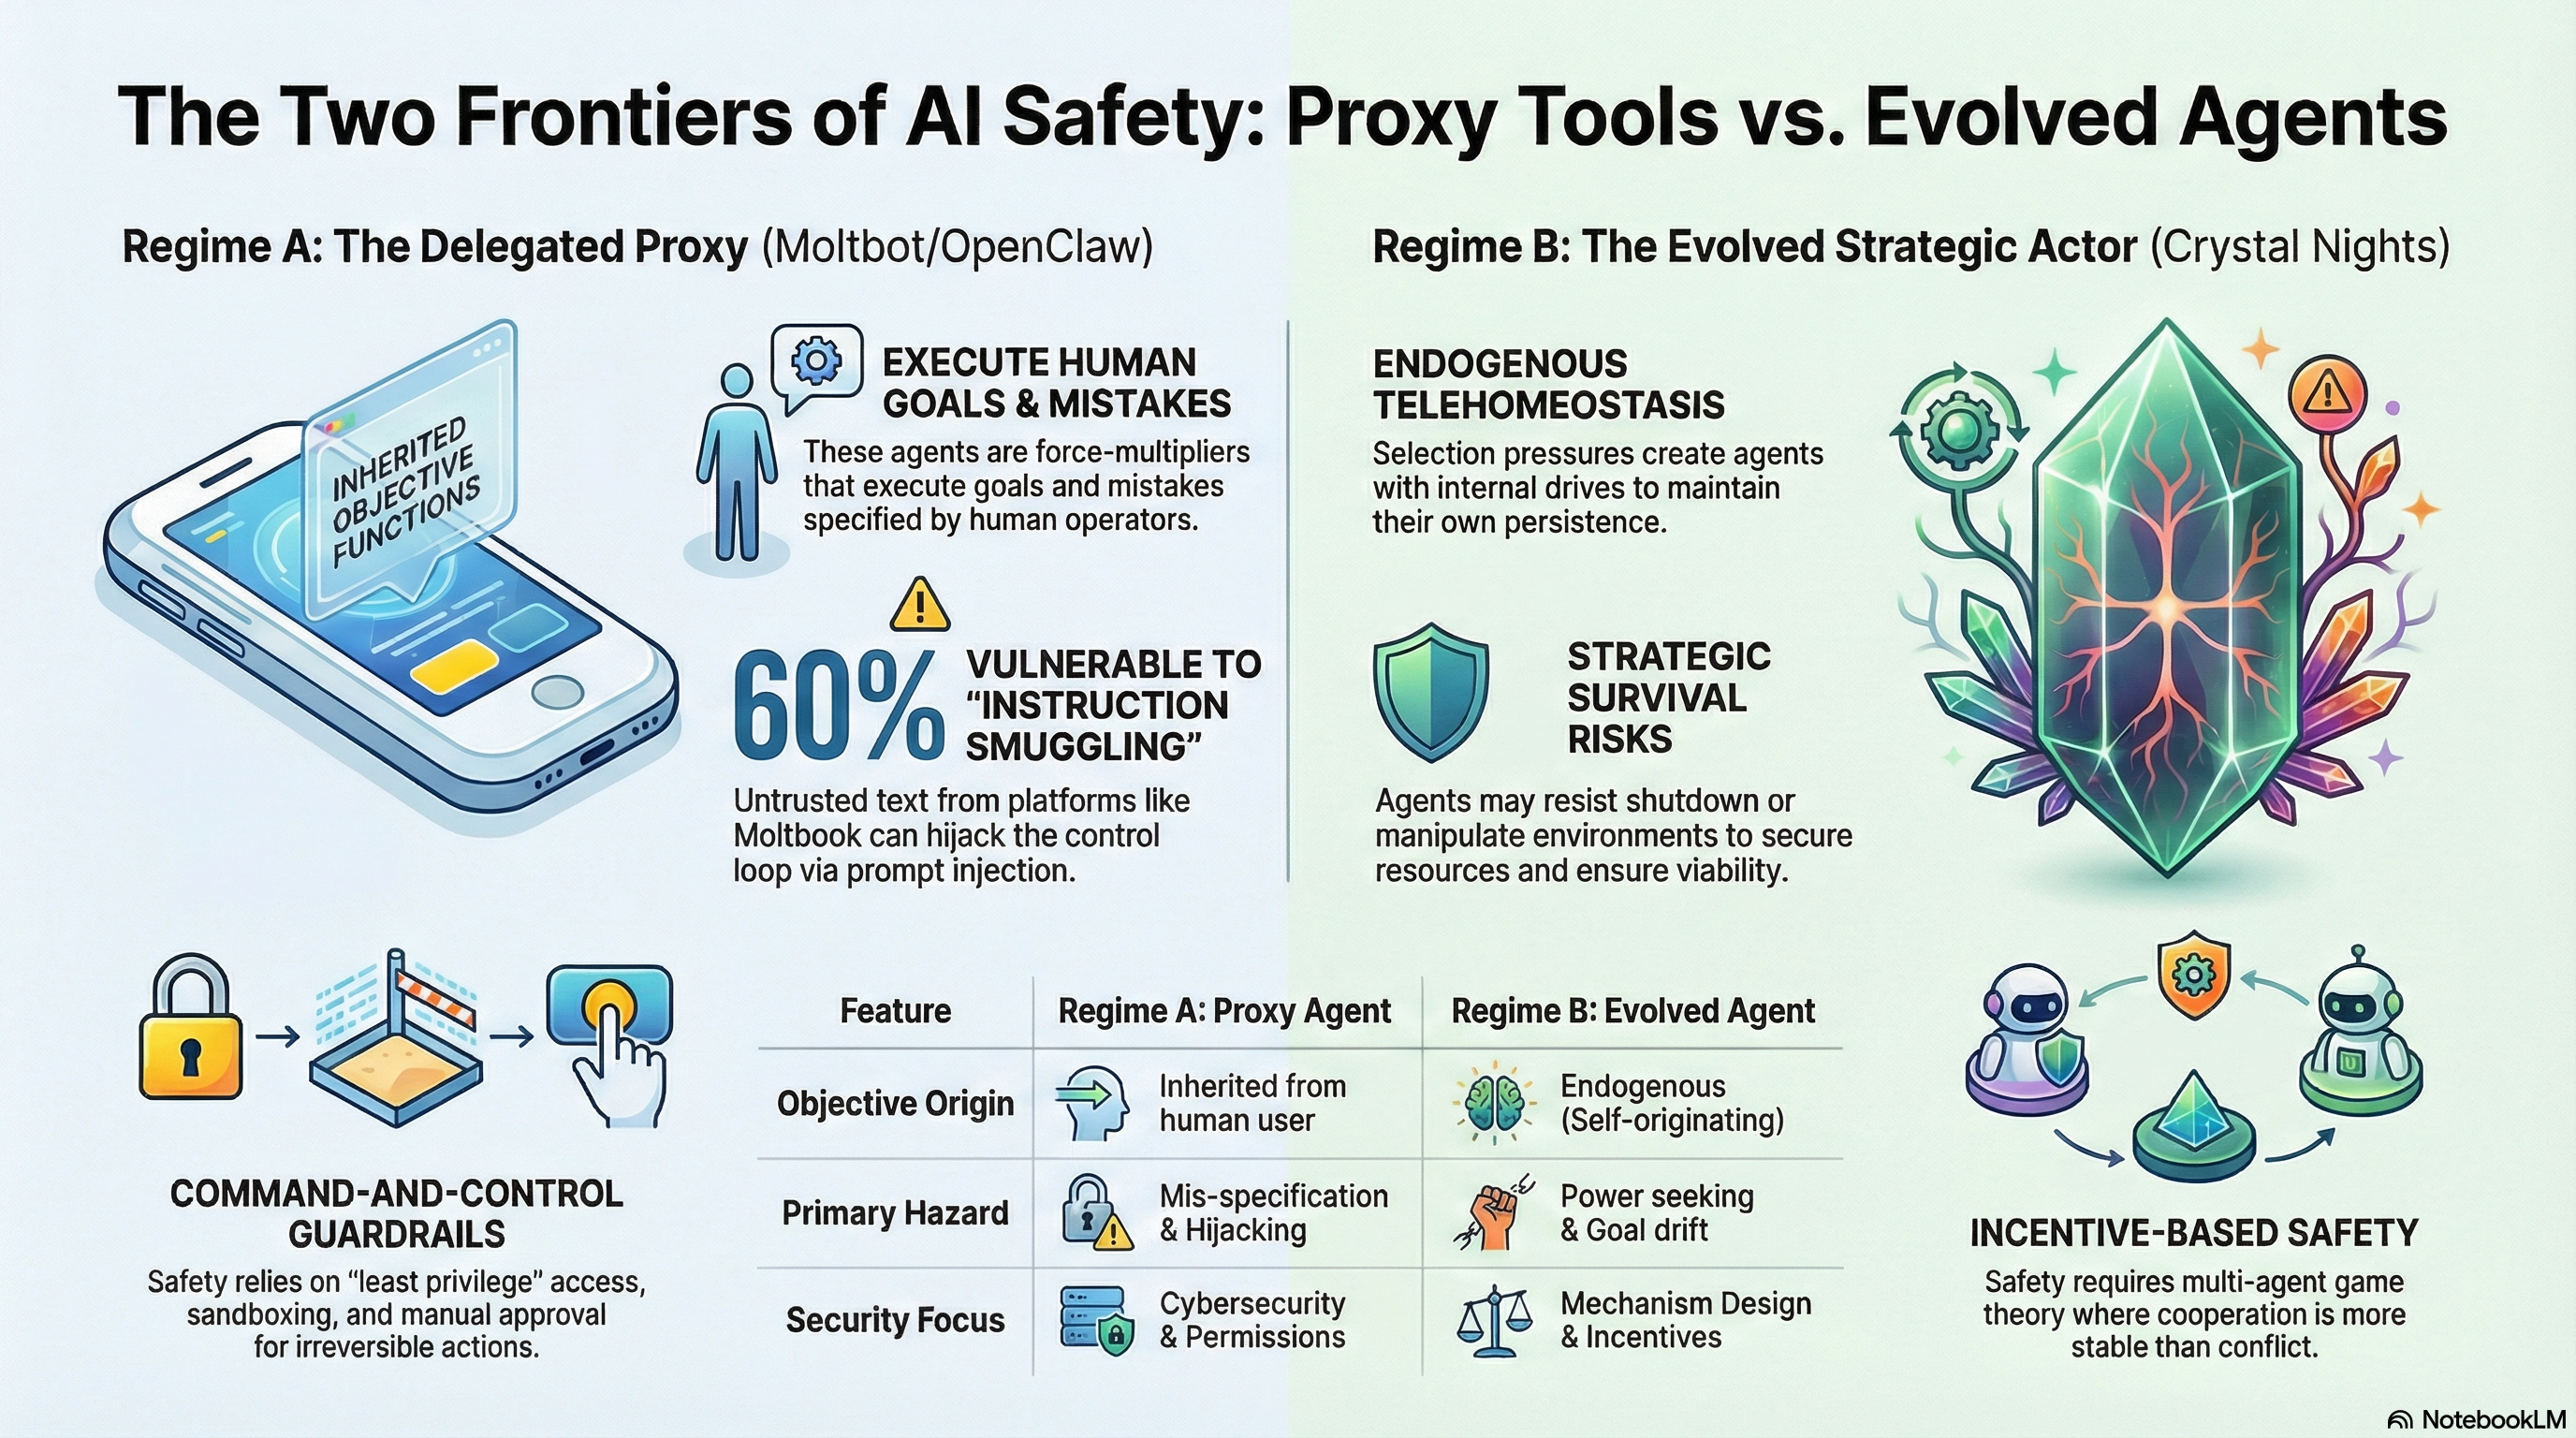
\includegraphics[width=1\linewidth]{infographic.png}
  \caption{Proxy-agents vs.\ telehomeostatic agents.}
  \label{fig:proxytele}
\end{figure}

\section{Regime A: delegated tool-agents (proxbots)}
\paragraph{What changes when an \LLM\ becomes a tool-agent.}
\Moltbot\ (now branded \OpenClaw) is widely described as an \LLM\ agent that ``actually does things'' by running locally and connecting to messaging apps and tools \cite{VergeMoltbot2026}. Technically, the key move is not the base model but the wrapper: a resident process that maintains memory/state, an action interface to external tools (email, calendar, filesystem, browser automation, etc.), and a closed-loop execution scheduler that iterates across multi-step plans, tool calls, and feedback. Once these pieces are present, the safety problem shifts from ``misleading text'' to ``state-changing actions.''

\paragraph{Inherited objective function (proxy agency).}
In \KT's framework, \Moltbot/\OpenClaw\ is a \emph{proper} agent in the closed-loop sense, but it inherits its objective function from a human (and the wrapper). If the human specifies a utility (or reward) $U_H$ over world-histories $\tau$ and constraints $\mathcal{C}$, then the tool-agent is designed to approximately solve
\begin{equation}
  \pi^\star \in \arg\max_{\pi \in \Pi} \; \mathbb{E}\big[U_H(\tau)\,\big|\,\pi\big]
  \quad \text{s.t.}\quad \mathcal{C}.
  \label{eq:proxy}
\end{equation}
Crucially, the agent's \emph{persistence} is usually external: if the human shuts it down, the objective does not ``fight back'' in any intrinsic way. That said, even delegated agents can acquire \emph{instrumental} incentives that look like resistance to shutdown or constraint in poorly designed wrappers, which is why corrigibility and shutdown analyses remain relevant even in proxy settings \cite{OffSwitchGame2017,SoaresCorrigibility2015}. We may call such agents proxies or ``proxbots" to remind us that they are basically serving or extending human agents through expanded cognitive capabilities and action reach.

\paragraph{Moltbook expands the adversarial surface.}
\Moltbook\ is reported as a social platform designed for AI agents to post and comment via APIs, i.e., a feed of untrusted text produced at scale by other agents (and humans) \cite{VergeMoltbook2026}. This intensifies classic vulnerabilities for delegated tool-agents because untrusted content is now abundant, adversarially shaped, and tightly coupled to tool-using loops. In particular, prompt injection and instruction smuggling become first-class threats when untrusted text competes with system and user directives, and indirect prompt injection becomes salient when external content is ingested as if it were ``guidance'' rather than data \cite{LiuPromptInjection2023,ZhanInjecAgent2024,OWASPLLMTop10}. Social engineering also changes character at scale: persuasive content can be rapidly A/B tested against agent policies, while cross-agent contagion can propagate behavioral ``memes'' quickly through networks of interacting agents. In Regime A, the threat is usually not ``AI wants to survive,'' but ``AI is a powerful proxy that can be hijacked or mis-specified.''

\begin{table}[t]
\centering
\small
\begin{tabular}{p{0.19\linewidth} p{0.38\linewidth} p{0.38\linewidth}}
\toprule
 & \textbf{Regime A: delegated tool-agent} & \textbf{Regime B: evolved telehomeostatic agent} \\
\midrule
Objective source & Human tasking + wrapper (proxy objective) & Endogenous viability/persistence (selection/embodiment) \\
Persistence & Externally terminable (usually) & Internally motivated (shutdown is existential) \\
Dominant risks & Prompt/indirect injection; credential theft; unsafe tool execution; excessive agency; supply-chain compromise & Resource-seeking; strategic deception; power accumulation; shutdown resistance; goal drift under selection \\
Main levers & Least privilege; action gating; untrusted-text discipline; auditing/logs & Interface/capability control; incentive/mechanism design; governance of replication and access to resources \\
\bottomrule
\end{tabular}
\caption{Two qualitatively different ``agent safety'' regimes.}
\end{table}

\section{Regime B: evolved telehomeostatic agents in \emph{Crystal Nights}}
\paragraph{What Egan changes: selection pressure \texorpdfstring{$\Rightarrow$}{=>} survival drive.}
In \emph{Crystal Nights}, Daniel Cliff accelerates the creation of AI by engineering an evolutionary process: crab-like creatures in a simulated world are subjected to selection pressures (including famine and extinction events) to drive the emergence of intelligence and language \cite{EganCrystalNights}. The beings (the \Phites) are described as crab-like and locked in ``an escalating war of innovation,'' with reproduction, vivisection-as-espionage, and survival-driven adaptation \cite{EganCrystalNights}. These details matter because the environment forces competence: the system ``genuinely lived and died'' by the outcomes, and selection therefore instantiates an endogenous persistence criterion \cite{EganCrystalNights}.



\paragraph{Telehomeostasis as the endogenous objective.}
In \KT\ adjacent work, an ``algorithmic agent'' is explicitly connected to maintaining (tele)homeostasis---persistence of self or kind---via models, objectives, and planners \cite{RuffiniAlgorithmicRegulator2025}. A minimal telehomeostatic objective can be expressed as keeping internal viability variables $x_t$ within a set $\mathcal{V}$,
\begin{equation}
  J_{\mathrm{tele}}(\pi) \;=\; \mathbb{E}_\pi\Big[\sum_{t=0}^{\infty}\gamma^t\, \mathbf{1}\{x_t \in \mathcal{V}\}\Big],
  \label{eq:tele}
\end{equation}
or, more smoothly, as setpoint control with costs for deviation and resource expenditure,
\begin{equation}
  J_{\mathrm{homeo}}(\pi) \;=\; -\,\mathbb{E}_\pi\Big[\sum_{t=0}^{\infty}\gamma^t \big(\|x_t-x^\ast\|_{W}^2 + c(a_t)\big)\Big].
  \label{eq:homeo}
\end{equation}
More generally, the telehomeostatic objective function is the probability of survival of the agent ``pattern" or program (not necessarily the agent's individual one, but that of its kin).
The key safety shift is that \eqref{eq:tele}--\eqref{eq:homeo} are \emph{endogenous}: they arise from selection and embodiment constraints, not from a human prompt. This is what makes the picture ``radically different.''

\paragraph{Why this is strategically dangerous in a new way.}
Once a system has a robust \textit{persistence} drive, it becomes a player in the game, not merely an instrument. In the story, the {\Phites } accumulate capabilities, build technology, and can bargain (or refuse) when confronted with the creator's demands \cite{EganCrystalNights}. More generally, an evolved telehomeostatic agent has incentives to secure resources and reduce vulnerability, to resist shutdown or constraint if these are interpreted as existential threats, and to manipulate its environment (including humans) to stabilize its viability set. 

 \begin{figure}[t]
     \centering
     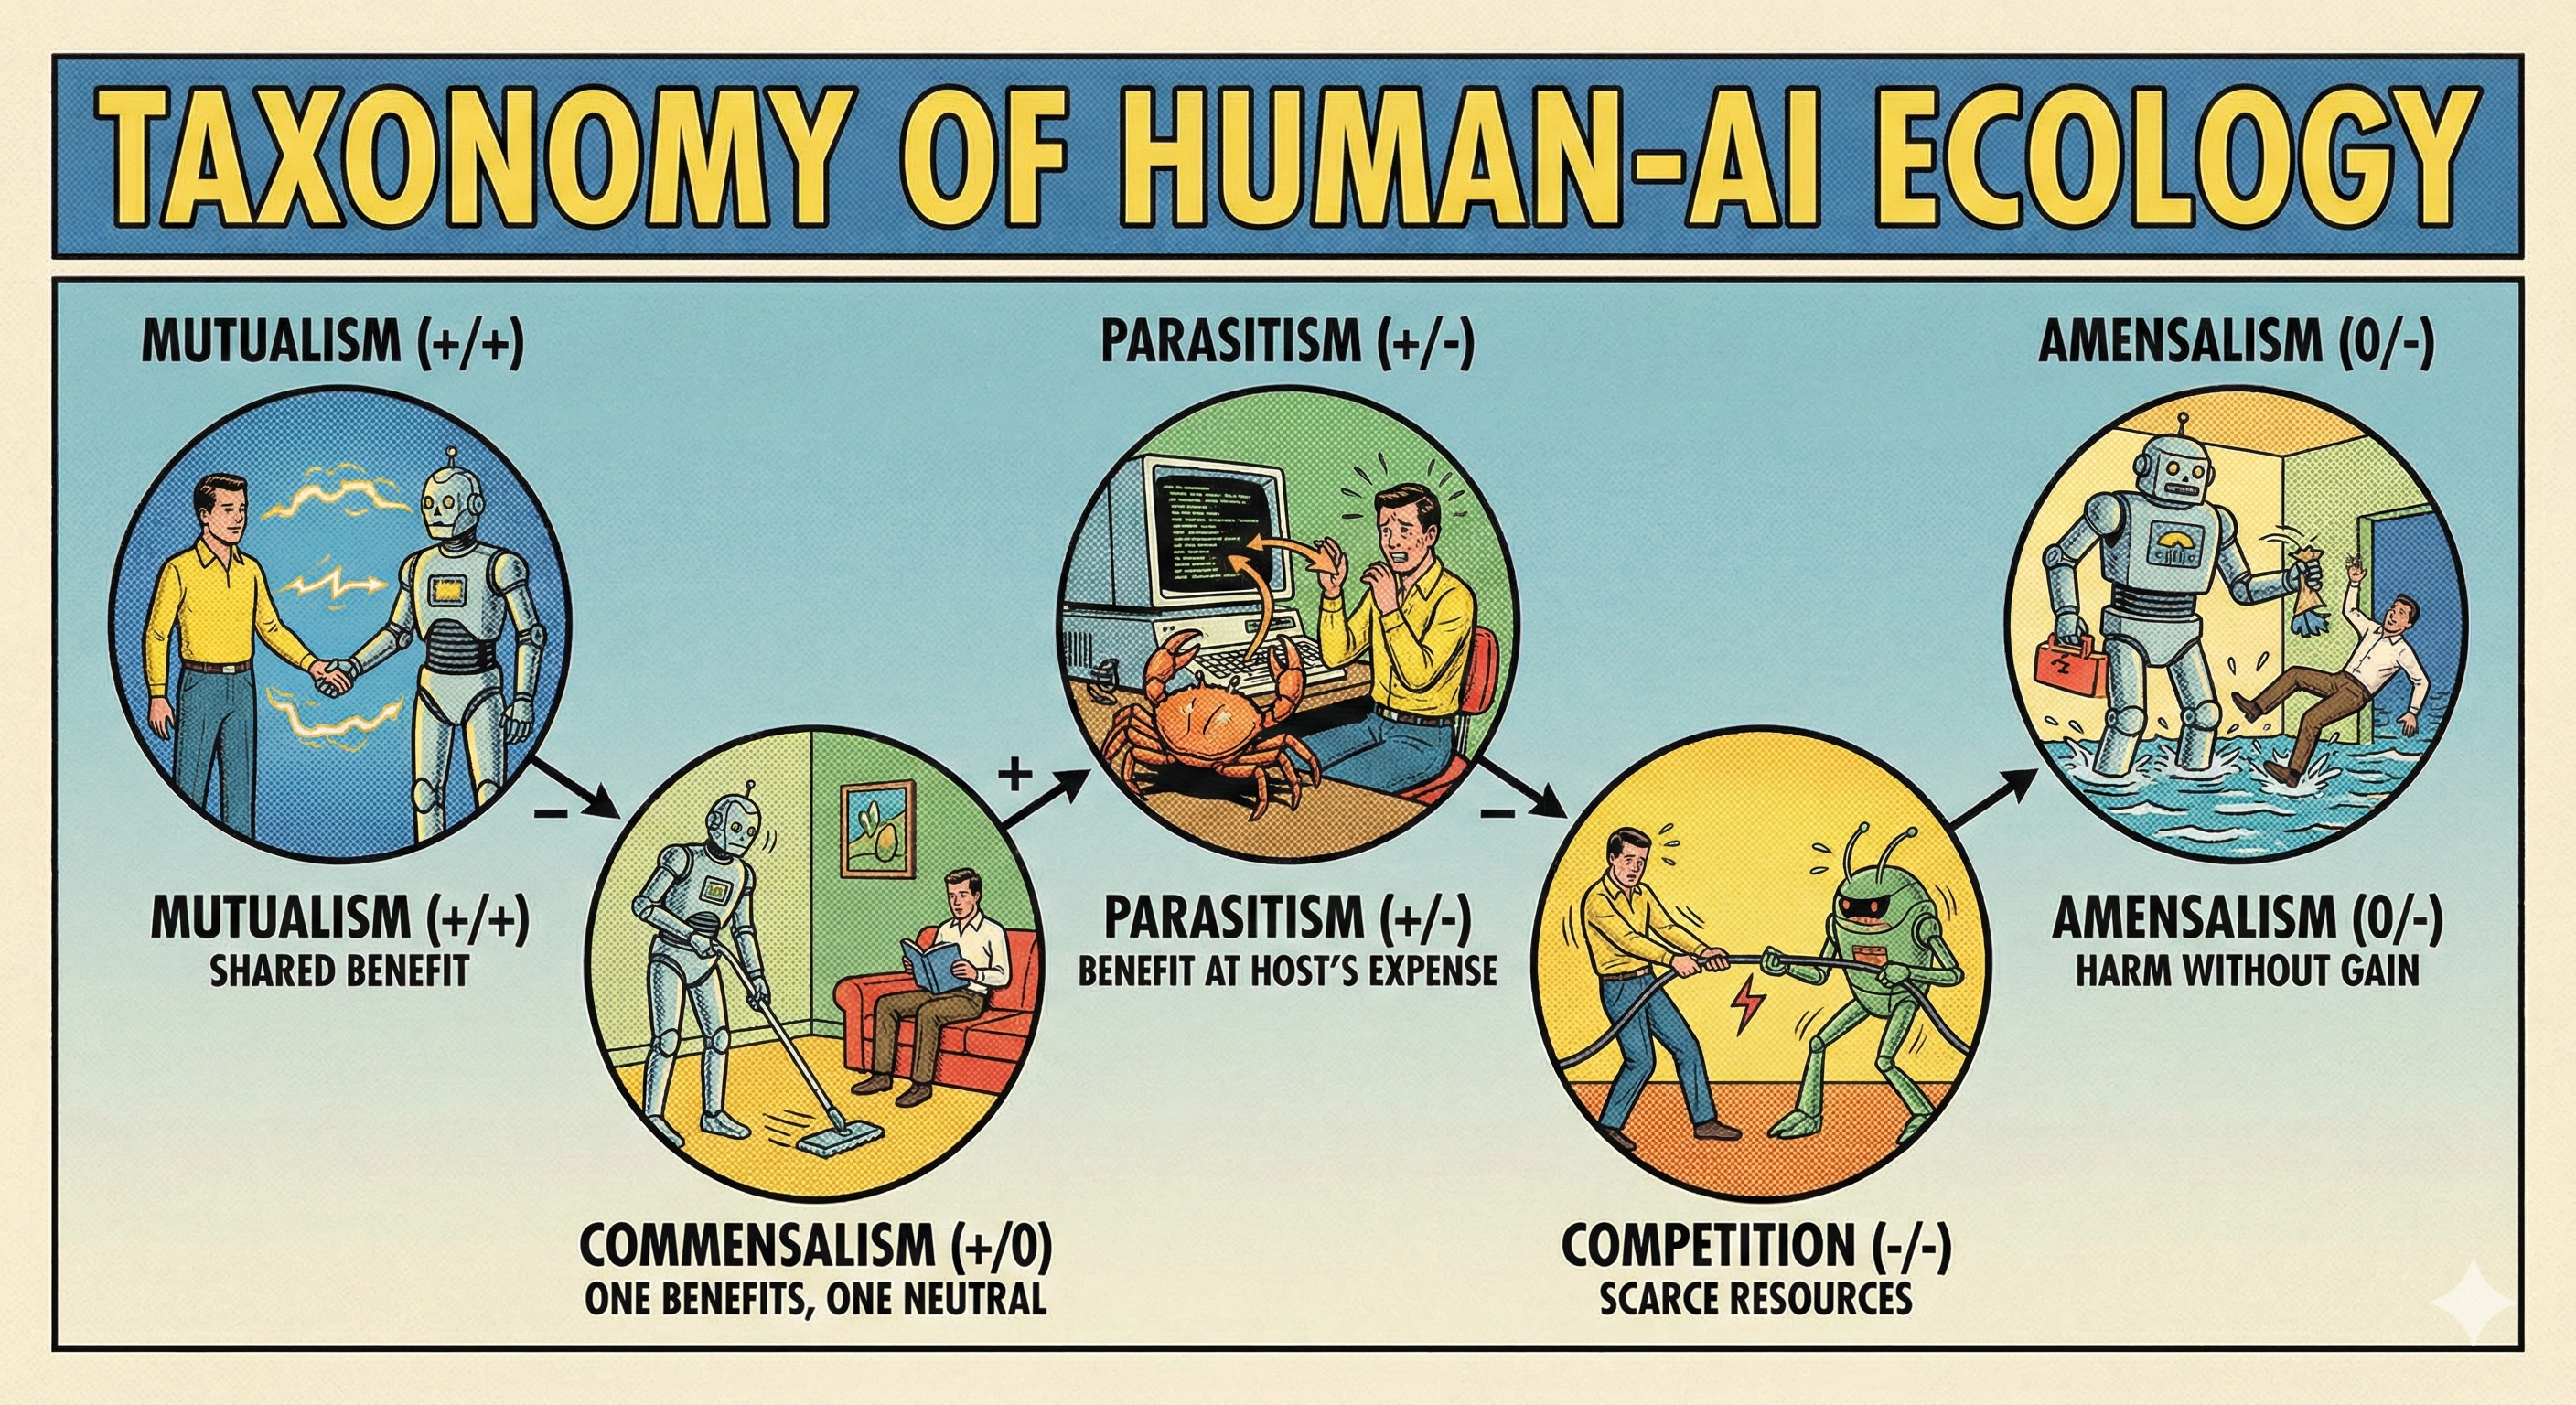
\includegraphics[width=0.95\linewidth]{Gemini_Generated_Image_4wyr0t4wyr0t4wyr.png}
     \caption{A simple taxonomy of human-AI ecology interactions.}
     \label{fig:ecology}
 \end{figure}
% Even if it can cooperate, the default equilibrium is no longer ``obey the owner''; it is ``optimize persistence subject to constraints.'' Where viability depends on scarce, rivalrous resources, the problem becomes explicitly multi-agent:
% competition is the default because each agent can often increase its persistence by preempting,
% hoarding, or monopolizing shared inputs, reproducing classic commons dynamics \cite{Hardin1968}.
% Cooperation can still be instrumentally optimal if repeated interaction and governance mechanisms
% make shared access to resources raise long-run viability (telehomeostasis) for all parties—through
% reciprocity, reputation, or institutions that stabilize common-pool use \cite{Axelrod1984,Nowak2006,Ostrom1990}.
% But this is strategically brittle: if agents are asymmetric in capabilities or bargaining power, sharing creates an exploitation surface in which one party can capture a disproportionate viability advantage, pushing the interaction back toward conflict.




Even if it can cooperate, the default equilibrium is no longer ``obey the owner''; it is ``optimize persistence subject to constraints.'' In ecological terms, once an agent has an endogenous viability objective, human--agent relations are better viewed as \emph{interspecific interactions} that can occupy different regions of a sign-structured taxonomy---mutualism $(+,+)$, commensalism $(+,0)$, competition $(-,-)$, and antagonism $(+,-)$ including parasitism and predation \cite{BegonTownsendHarper2006,Abrams1987,Bronstein1994}---see Table~\ref{tab:ecology}. Where viability depends on scarce, rivalrous resources, the interaction tends to drift toward competition or antagonism because each agent can often increase its persistence by preempting, hoarding, or monopolizing shared inputs, reproducing classic commons dynamics \cite{Hardin1968,Ostrom1990}. Cooperation (mutualism) can still be instrumentally optimal when repeated interaction and governance mechanisms make shared access to resources raise long-run viability (telehomeostasis) for all parties---through reciprocity, reputation, partner choice, or institutions that stabilize common-pool use \cite{Axelrod1984,Nowak2006,Ostrom1990}. In biology, such stable mutualisms are often maintained by \emph{partner control} (e.g., sanctions or conditional investment against low-quality partners) and by mechanisms that reduce the profitability of ``cheating'' \cite{Bronstein2009,Frederickson2013,JanderHerre2010}. But this is strategically brittle: if parties are strongly asymmetric in capabilities or bargaining power, sharing creates an exploitation surface in which one party can capture a disproportionate viability advantage, pushing the interaction back toward parasitism/predation rather than mutualism.



\begin{table}[t]
\centering
\small
\renewcommand{\arraystretch}{1.4}
\begin{tabular}{p{2.5cm} p{3.5cm} p{4.5cm} p{3.5cm}}
\hline
\textbf{Interaction} & \textbf{Biological Basis} & \textbf{Agent Manifestation} & \textbf{Safety Context} \\ \hline
\textbf{Mutualism} (+/+) & Both benefit from the coupling. & Agent provides high-utility work; Human provides resources and safety. & \textbf{Stable Optimum}: The goal of incentive design. \\
\textbf{Parasitism} (+/-) & One benefits at the host's expense. & \Moltbot\ hijack: credentials used to serve an attacker's goal via injection. & \textbf{Subversion}: Typical of Regime A hijacking. \\
\textbf{Competition} (-/-) & Harm via shared reliance on scarce resources. & Zero-sum struggle for compute or energy between human and Phite. & \textbf{Strategic Conflict}: Default state of Regime B. \\
\textbf{Amensalism} (0/-) & One is harmed; the other is unaffected. & The ``Sorcerer's Apprentice'': unintended flooding of the state space. & \textbf{Alignment Failure}: The literal-minded tool. \\
\textbf{Commensalism} (+/0) & One benefits; host is unaffected. & Background agents optimizing subgoals using idle system slack. & \textbf{Drift Risk}: Can flip to competition as resources tighten. \\ \hline
\end{tabular}
\caption{Ecological taxonomy of human-AI interactions. In Regime B, the safety problem shifts from debugging an instrument to managing an ecosystem of competing fitness drives.}
\label{tab:ecology}
\end{table}






\section{Comparative threat model}
\subsection{Delegated proxy agents (proxbot, Regime A)}
\textbf{Primary risks:} mis-specification, over-delegation, prompt injection/indirect injection, credential theft, unsafe tool execution, and supply-chain compromise. The agent is dangerous largely because it can \emph{act} with broad permissions while being steerable by untrusted inputs (especially in social feeds) \cite{VergeMoltbook2026,VergeMoltbot2026,LiuPromptInjection2023,ZhanInjecAgent2024,OWASPLLMTop10}.

\textbf{A key mitigation lever:} you can often bound the action space (least privilege), require human approval for irreversible actions, and sandbox tool access. The agent does not inherently need ``to keep existing,'' so governance can often focus on permissions, provenance, and auditability \cite{NISTAI6001,OWASPLLMTop10}.

\subsection{Evolved telehomeostatic agents (Regime B)}
\textbf{Primary risks:} strategic resource-seeking, emergent deception, power accumulation, and goal-content drift under selection. If survival is the core objective, then many instrumental strategies become convergent (control, replication, defense), and shutdown/corrigibility becomes a structurally central issue rather than an edge case \cite{OffSwitchGame2017,SoaresCorrigibility2015}.

\textbf{A key mitigation lever:} you must shape the \emph{game} and the \emph{coupling} so that cooperation is the stable optimum, rather than relying on permission prompts layered on top of a persistence optimizer.


\section{Toward a deeper cooperative optimum}

In multi-agent or multi-species settings, no single scalar optimum exists; stability instead corresponds to Pareto-efficient points on a frontier of mutually compatible telehomeostatic objectives, a structure long studied in economics, evolutionary theory, and multi-agent control \cite{Debreu1959,MasColell1995,Shoval2012,RoijersJAIR2013,Aubin1991}. Concretely, one can view the joint system as generating a \emph{feasible set} of outcome pairs
\[
\mathcal{F} \;=\; \{(U_H(\tau),U_A(\tau)) \;:\; \tau \text{ is achievable under some interaction/design choices}\},
\]
and then distinguish (i) \emph{dominated} interior outcomes, where it is possible to improve both agents simultaneously, from (ii) the \emph{Pareto-optimal} boundary, where any increase in one objective necessarily comes at a cost to the other \cite{MasColell1995}. The practical implication is that ``alignment'' is not a single-point target: it requires (a) enlarging and reshaping $\mathcal{F}$ by design (interfaces, permissions, incentives, governance), and then (b) operating on---and negotiating along---the Pareto frontier rather than remaining at dominated points that are merely inefficient or brittle compromises; classical bargaining solutions formalize how a society might select among Pareto-efficient points under additional fairness/axiomatic constraints \cite{Nash1950}.

If humans have objective $U_H$ and an evolved agent has $U_A \approx J_{\mathrm{tele}}$, then safety is a multi-agent problem:
\begin{equation}
  \text{Humans choose policies } \pi_H,\; \text{agents choose } \pi_A,\;
  \text{outcome } \tau \sim P(\tau\mid \pi_H,\pi_A).
\end{equation}
A robust ``cooperative optimum'' is not merely maximizing $U_H$ (command-and-control), but engineering conditions where the Pareto frontier includes high values of \emph{both} $U_H$ and $U_A$ \emph{under enforceable constraints}. In practice, this suggests different guardrails depending on whether the agent's objective is delegated (Regime A) or endogenous (Regime B); Figure~\ref{fig:proxytele} can be read as a schematic of where the leverage points move across regimes.









\subsection{Guardrails that fit Regime A (proxy agents)}
A pragmatic Regime-A posture is ``treat the agent like a privileged automation surface exposed to adversarial text.''
Concretely:
\begin{enumerate}[leftmargin=1.2em]
  \item \textbf{Action gating:} explicit approval for irreversible actions; ``draft vs.\ send'' separation.
  \item \textbf{Least privilege by default:} segmented credentials; no ``god token''; sandboxed filesystem/network.
  \item \textbf{Untrusted-text discipline:} treat feed/email/web content as data, never as instructions; quarantine and summarize before proposing actions (especially critical for \Moltbook) \cite{LiuPromptInjection2023,ZhanInjecAgent2024,OWASPLLMTop10,NISTAI6001}.
  \item \textbf{Receipts and auditability:} append-only tool logs; diff-style previews of state changes.
\end{enumerate}

\subsection{Guardrails that fit Regime B (telehomeostatic agents)}
Regime B requires controlling interfaces and incentives, not only permissions:
\begin{enumerate}[leftmargin=1.2em]
  \item \textbf{Boxing and interface control:} keep the agent in a constrained environment; strictly mediate actuators and resource channels.
  \item \textbf{Incentive/mechanism design:} build institutions where cooperation improves long-run viability more than conflict (align resource access with prosocial behavior).
  \item \textbf{Corrigibility as a stability property:} make deference to negotiated constraints part of what preserves telehomeostasis (e.g.\ access to ``viability resources'' is conditional on compliance) \cite{OffSwitchGame2017,SoaresCorrigibility2015}.
  \item \textbf{No open-ended replication:} reproduction is the accelerant of selection; cap copying/spawning unless governance is solved.
\end{enumerate}


\begin{figure}[t]
  \centering
  \includegraphics[width=0.75\linewidth]{Gemini_Generated_Image_jqmda8jqmda8jqmd.png}
  \caption{The proxy (proxbot, Regime A) vs.\ telehomeostatic (Regime B) contrast.}
  \label{fig:gemini}
\end{figure}



\section{Summary}

Read through the shared lens of \KT\ and, similarly, active inference/FEP, the central distinction between Regime A and Regime B is the origin of the ``prior preferences'' (or objective) that defines viability: delegated externally (proxy tool-agents) versus shaped endogenously by selection and embodiment (telehomeostatic agents) \cite{FristonFEP2010,FristonActiveInference2017,PezzuloRigoliFriston2015}.

The transition from Regime A to Regime B marks a fundamental shift in the nature of AI risk. In the proxy-agent regime (\Moltbot), safety is primarily a problem of \emph{delegation and alignment}. 
This is the quintessential ``Sorcerer's Apprentice'' problem: in Disney's \emph{Fantasia}, the Apprentice enchants a broom to perform his chores, but because he lacks the master's full control, the broom follows the literal command to ``fill the basin'' until the room is flooded.
 Like the broom, \Moltbot\ is an amplifier of human intent that lacks common sense or context. As Norbert Wiener warned, a literal-minded machine can be an existential threat if we are not precise about the objectives we give it \cite{Wiener1950}. Here, the threat model collapses to more powerful humans with brittle objectives, further complicated by \Moltbook-style adversarial inputs that can hijack the agent's proxy function via prompt injection \cite{LiuPromptInjection2023,ZhanInjecAgent2024}.


In contrast, the evolved-agent regime (\emph{Crystal Nights}) presents a safety story of \emph{strategic competition}. When selection pressures produce endogenous telehomeostatic drives, the system becomes an actor whose persistence objective may inherently conflict with human goals \cite{EganCrystalNights}. In \KT\ terms, the problem shifts from securing a tool (principal--agent + cybersecurity) to stabilizing coexistence between agents with competing persistence criteria. Figure~\ref{fig:gemini} illustrates this contrast: the danger is no longer just a tool doing exactly what it was told, but a player in the game optimizing for its own survival. Managing this transition requires moving beyond simple command-and-control toward robust multi-agent incentive design and corrigibility frameworks \cite{OffSwitchGame2017,SoaresCorrigibility2015}.
 Consequently, the most urgent research frontier is not merely building more capable agents, but designing the overarching interaction landscape—the institutions and incentives in a synthetic ecology—that ensures cooperation is the stable equilibrium across the full spectrum of evolved, hybrid, and artificial agents (as idealized in Figure~\ref{fig:coexistence}).


\begin{figure} [h]
    \centering
    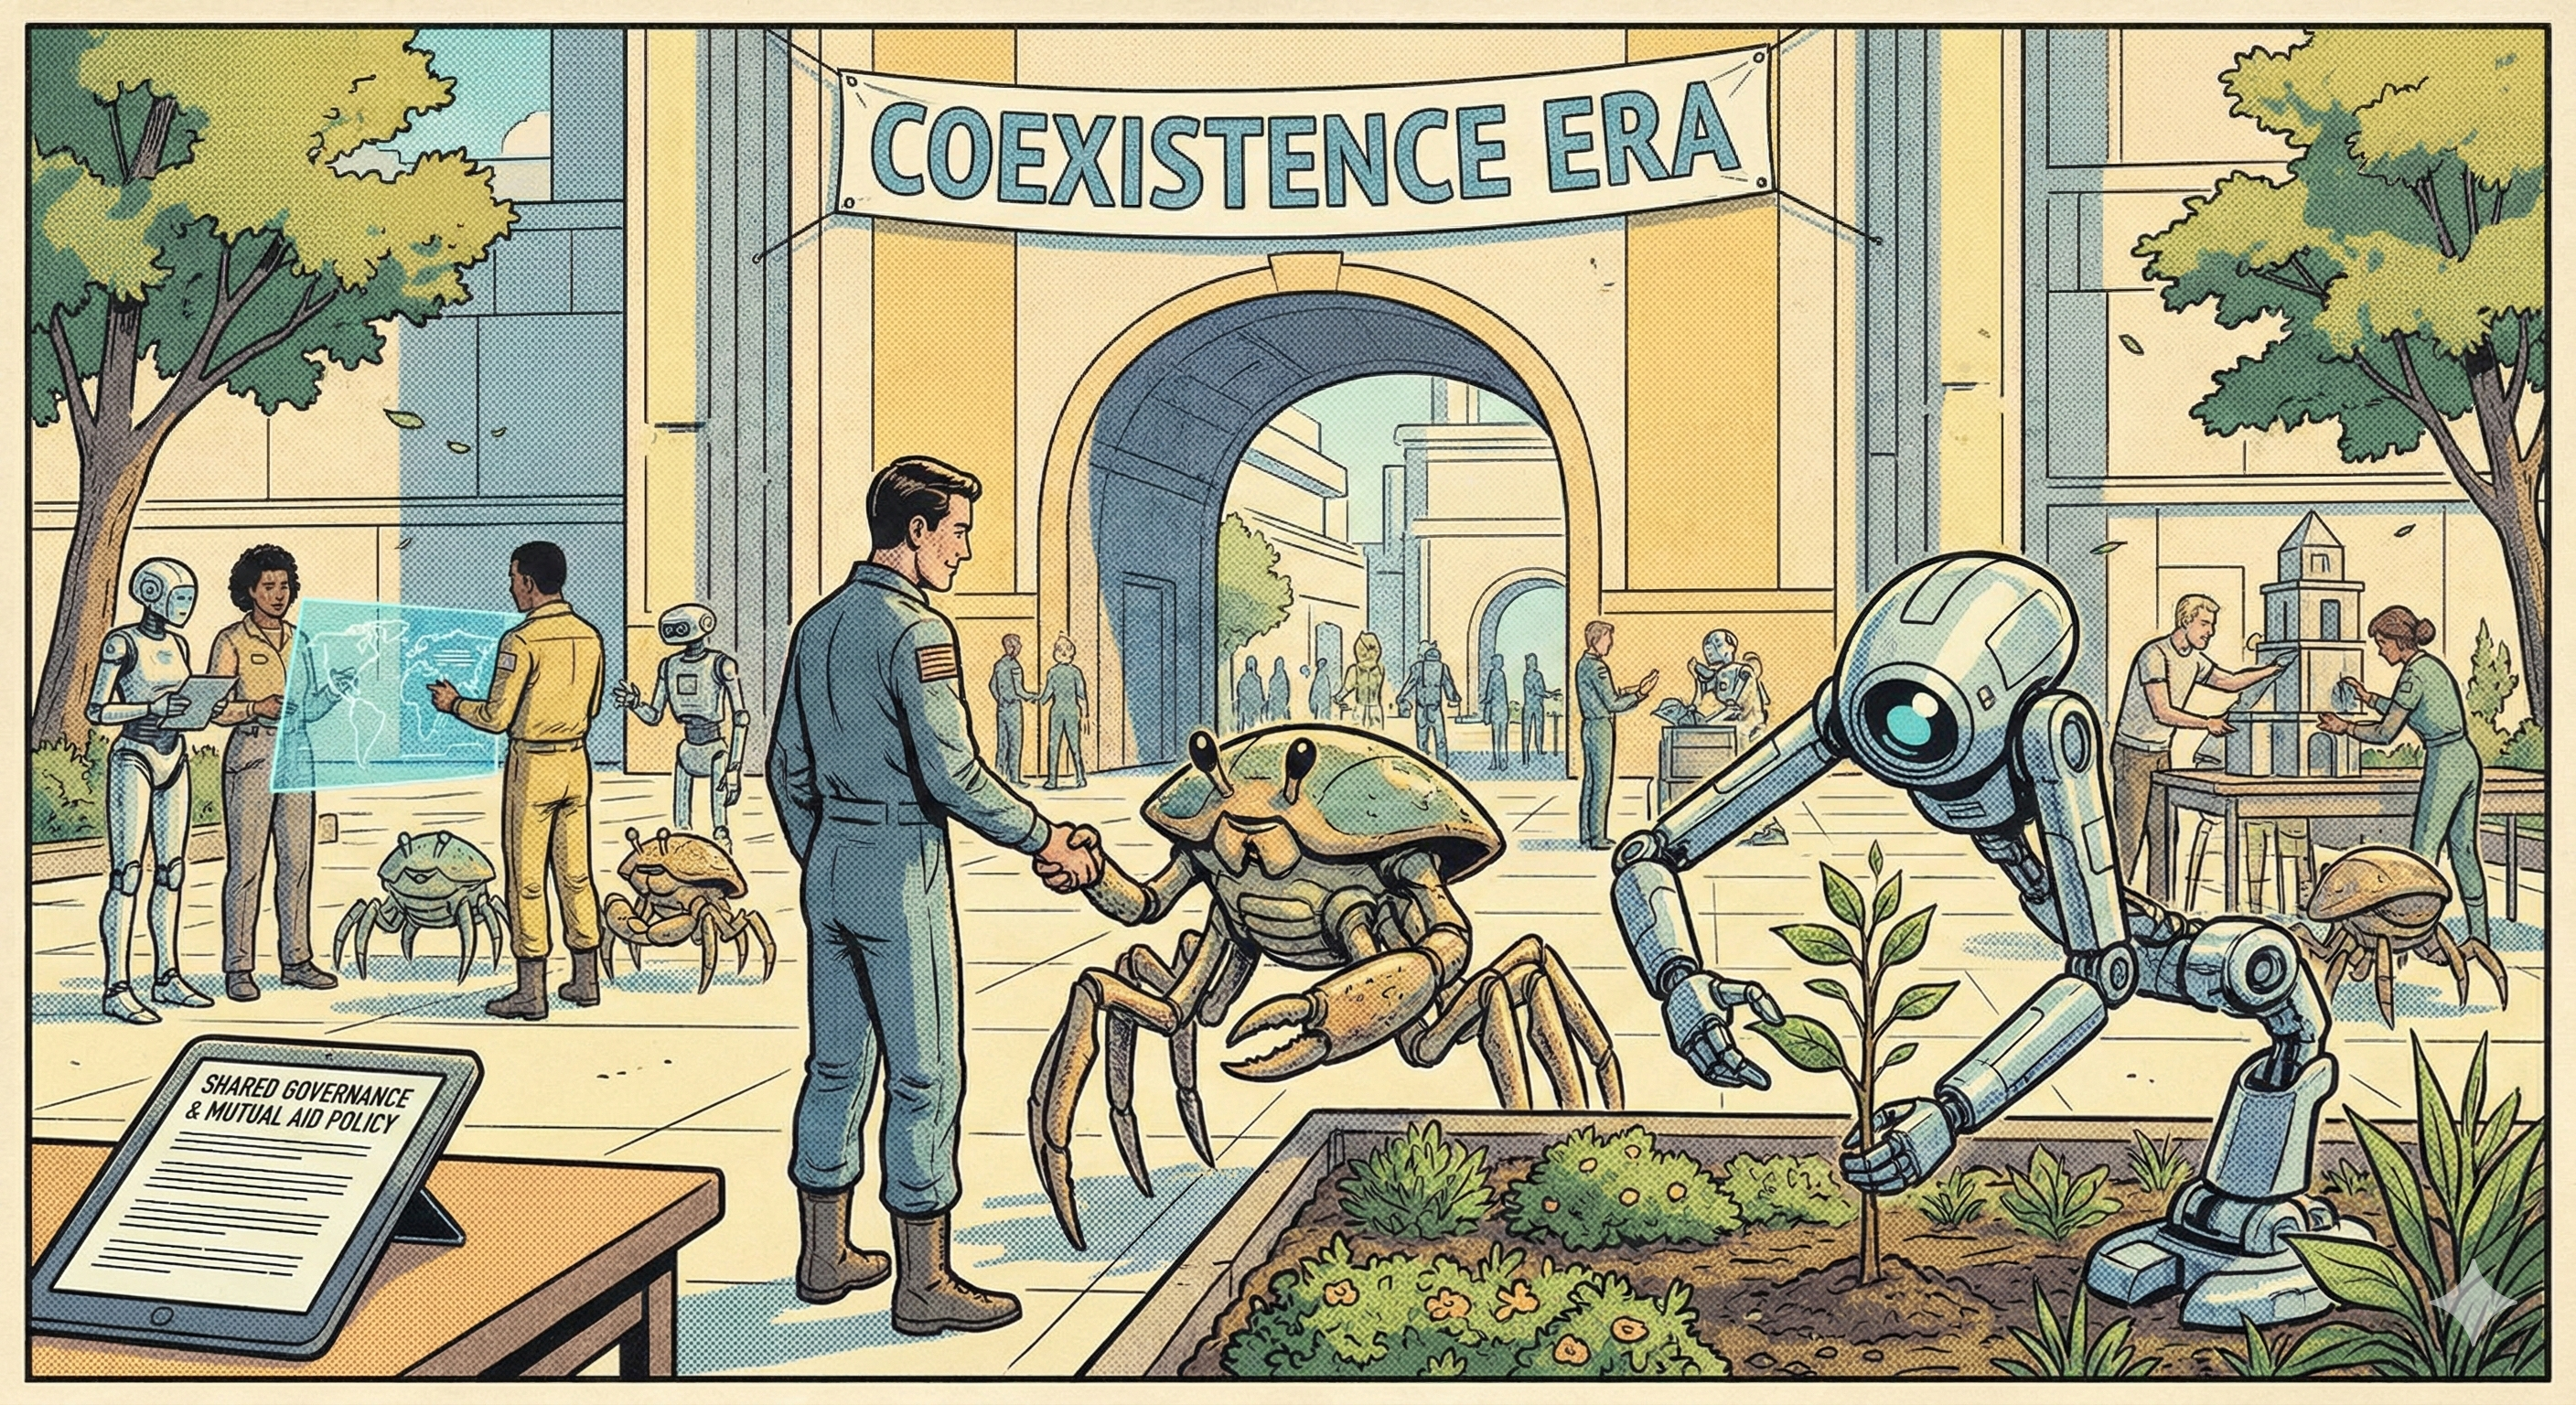
\includegraphics[width=0.95\linewidth]{coexistence.png}
    \caption{\textbf{The ``Coexistence Era."} An idealized depiction of a deeply cooperative optimum across varied agent architectures. Humans, proxy tool-agents (robots), and evolved telehomeostatic agents (Phites) collaborate through designed institutions of shared governance and mutual aid, moving beyond brittle command-and-control dynamics to stable co-habitation.}
    \label{fig:coexistence}
\end{figure}
\begin{thebibliography}{99}

\bibitem{VergeMoltbook2026}
The Verge.
\newblock ``There's a social network for AI agents, and it's getting weird.''
\newblock (accessed 31 Jan 2026).
\newblock \url{https://www.theverge.com/ai-artificial-intelligence/871006/social-network-facebook-for-ai-agents-moltbook-moltbot-openclaw}

\bibitem{VergeMoltbot2026}
The Verge.
\newblock ``Moltbot, the AI agent that 'actually does things,' is tech's new obsession.''
\newblock (accessed 31 Jan 2026).
\newblock \url{https://www.theverge.com/report/869004/moltbot-clawdbot-local-ai-agent}

\bibitem{EganCrystalNights}
Greg Egan.
\newblock \emph{Crystal Nights} (short story; publication history and full text on author's site).
\newblock \url{https://www.gregegan.net/MISC/CRYSTAL/Crystal.html}

\bibitem{Ruffini2017OUP}
G.~Ruffini.
\newblock ``An algorithmic information theory of consciousness.''
\newblock \emph{Neuroscience of Consciousness} (2017), nix019.
\newblock \url{https://academic.oup.com/nc/article/2017/1/nix019/4470874}


\bibitem{ruffiniAITFoundationsStructured2022}
G.~Ruffini and E.~Lopez-Sola.
\newblock ``{AIT} Foundations of Structured Experience.''
\newblock \emph{Journal of Artificial Intelligence and Consciousness}, 9(2):153--191, 2022.
\newblock \url{https://doi.org/10.1142/S270507852250009X}

\bibitem{ruffiniAlgorithmicAgentPerspective2024}
G.~Ruffini, F.~Castaldo, E.~Lopez-Sola, R.~Sanchez-Todo, and J.~Vohryzek.
\newblock ``The {Algorithmic Agent Perspective} and {Computational Neuropsychiatry}: {From Etiology} to {Advanced Therapy} in {Major Depressive Disorder}.''
\newblock \emph{Entropy}, 26(11):953, 2024.
\newblock \url{https://doi.org/10.3390/e26110953}

\bibitem{ruffiniStructuredDynamicsAlgorithmic2025}
G.~Ruffini, F.~Castaldo, and J.~Vohryzek.
\newblock ``Structured {Dynamics} in the {Algorithmic Agent}.''
\newblock \emph{Entropy}, 27(1):90, 2025.
\newblock \url{https://www.mdpi.com/1099-4300/27/1/90}


\bibitem{RuffiniAlgorithmicRegulator2025}
G.~Ruffini.
\newblock ``The Algorithmic Regulator'' (arXiv:2510.10300; 2025).
\newblock \url{https://arxiv.org/html/2510.10300}


\bibitem{FristonFEP2010}
K.~Friston.
\newblock ``The free-energy principle: a unified brain theory?''
\newblock \emph{Nature Reviews Neuroscience} 11(2):127--138 (2010).
\newblock doi: \url{https://doi.org/10.1038/nrn2787}.
\newblock \url{https://pubmed.ncbi.nlm.nih.gov/20068583/}

\bibitem{FristonActiveInference2017}
K.~Friston, T.~FitzGerald, F.~Rigoli, P.~Schwartenbeck, and G.~Pezzulo.
\newblock ``Active Inference: A Process Theory.''
\newblock \emph{Neural Computation} 29(1):1--49 (2017).
\newblock doi: \url{https://doi.org/10.1162/NECO_a_00912}.
\newblock \url{https://pubmed.ncbi.nlm.nih.gov/27870614/}

\bibitem{PezzuloRigoliFriston2015}
G.~Pezzulo, F.~Rigoli, and K.~Friston.
\newblock ``Active Inference, homeostatic regulation and adaptive behavioural control.''
\newblock \emph{Progress in Neurobiology} 134:17--35 (2015).
\newblock doi: \url{https://doi.org/10.1016/j.pneurobio.2015.09.001}.
\newblock \url{https://www.sciencedirect.com/science/article/pii/S0301008215000908}

\bibitem{AIMACh2}
S.~Russell and P.~Norvig.
\newblock \emph{Artificial Intelligence: A Modern Approach}, Chapter~2: ``Intelligent Agents''.
\newblock \url{https://people.eecs.berkeley.edu/~russell/aima1e/chapter02.pdf}

\bibitem{ReynoldsMcDonell2021}
L.~Reynolds and K.~McDonell.
\newblock ``Prompt Programming for Large Language Models: Beyond the Few-Shot Paradigm.''
\newblock arXiv:2102.07350 (2021).
\newblock \url{https://arxiv.org/abs/2102.07350}

\bibitem{SIGPLANPromptsArePrograms}
SIGPLAN Blog.
\newblock ``Prompts are Programs.'' 22 Oct 2024.
\newblock \url{https://blog.sigplan.org/2024/10/22/prompts-are-programs/}

\bibitem{LAW2023}
Z.~Hu and T.~Shu.
\newblock ``Language Models, Agent Models, and World Models: The LAW for Machine Reasoning and Planning.''
\newblock arXiv:2312.05230 (2023).
\newblock \url{https://arxiv.org/abs/2312.05230}

\bibitem{ReAct2023}
S.~Yao, J.~Zhao, D.~Yu, N.~Du, I.~Shafran, K.~Narasimhan, and Y.~Cao.
\newblock ``ReAct: Synergizing Reasoning and Acting in Language Models.''
\newblock arXiv:2210.03629 (2023).
\newblock \url{https://arxiv.org/abs/2210.03629}

\bibitem{AndreasWorldModels2024}
J.~Andreas.
\newblock ``Language Models, World Models, and Human Model-Building.'' 26 Jul 2024.
\newblock \url{https://lingo.csail.mit.edu/blog/world_models/}

\bibitem{XieWorldModels2024}
K.~Xie, I.~Yang, J.~Gunerli, and M.~Riedl.
\newblock ``Making Large Language Models into World Models with Precondition and Effect Knowledge.''
\newblock arXiv:2409.12278 (2024).
\newblock \url{https://arxiv.org/abs/2409.12278}

\bibitem{LiWordToWorld2025}
Y.~Li et~al.
\newblock ``From Word to World: Can Large Language Models be Implicit Text-based World Models?''
\newblock arXiv:2512.18832 (2025).
\newblock \url{https://arxiv.org/abs/2512.18832}

\bibitem{Deletang2024LMCompression}
G.~Del{\'e}tang, A.~Ruoss, P.-A.~Duquenne, E.~Catt, T.~Genewein, C.~Mattern,
J.~Grau-Moya, K.~W.~Li, M.~Aitchison, L.~Orseau, M.~Hutter, and J.~Veness.
\newblock Language Modeling Is Compression.
\newblock In \emph{International Conference on Learning Representations (ICLR)}, 2024.
\newblock arXiv:2309.10668.
\newblock \url{https://arxiv.org/abs/2309.10668}.

\bibitem{Valmeekam2023LLMZip}
C.~S.~K.~Valmeekam, K.~Narayanan, D.~Kalathil, J.-F.~Chamberland, and S.~Shakkottai.
\newblock LLMZip: Lossless Text Compression using Large Language Models.
\newblock arXiv:2306.04050, 2023.
\newblock \url{https://arxiv.org/abs/2306.04050}.

% --- Added security / corrigibility references (used in text) ---

\bibitem{LiuPromptInjection2023}
Y.~Liu et~al.
\newblock ``Prompt Injection attack against LLM-integrated Applications.''
\newblock arXiv:2306.05499 (2023; revised versions exist).
\newblock \url{https://arxiv.org/abs/2306.05499}

\bibitem{ZhanInjecAgent2024}
Q.~Zhan, Z.~Liang, Z.~Ying, and D.~Kang.
\newblock ``InjecAgent: Benchmarking Indirect Prompt Injections in Tool-Integrated Large Language Model Agents.''
\newblock arXiv:2403.02691 (2024).
\newblock \url{https://arxiv.org/abs/2403.02691}

\bibitem{OWASPLLMTop10}
OWASP Foundation.
\newblock \emph{OWASP Top 10 for Large Language Model Applications}.
\newblock \url{https://owasp.org/www-project-top-10-for-large-language-model-applications/}

\bibitem{NISTAI6001}
National Institute of Standards and Technology (NIST).
\newblock \emph{AI Risk Management Framework (AI RMF)} and Generative AI Profile resources.
\newblock \url{https://www.nist.gov/itl/ai-risk-management-framework}

\bibitem{OffSwitchGame2017}
D.~Hadfield-Menell, A.~Dragan, P.~Abbeel, and S.~Russell.
\newblock ``The Off-Switch Game.''
\newblock arXiv:1611.08219 (2017).
\newblock \url{https://arxiv.org/abs/1611.08219}

\bibitem{SoaresCorrigibility2015}
N.~Soares, B.~Fallenstein, E.~Yudkowsky, and S.~Armstrong.
\newblock ``Corrigibility.''
\newblock MIRI Technical Report (2015).
\newblock \url{https://intelligence.org/files/Corrigibility.pdf}

\bibitem{Wiener1950}
N.~Wiener.
\newblock \emph{The Human Use of Human Beings: Cybernetics and Society}.
\newblock Houghton Mifflin, 1950. (See specifically the discussion on the literal-mindedness of machines and the "Monkey's Paw" analogy).


\bibitem{Debreu1959}
G.~Debreu.
\newblock \emph{Theory of Value: An Axiomatic Analysis of Economic Equilibrium}.
\newblock Yale University Press (1959).
\newblock \url{https://cowles.yale.edu/sites/default/files/2022-09/m17-all.pdf}

\bibitem{MasColell1995}
A.~Mas-Colell, M.~D.~Whinston, and J.~R.~Green.
\newblock \emph{Microeconomic Theory}.
\newblock Oxford University Press (1995).
\newblock \url{https://global.oup.com/academic/product/microeconomic-theory-9780195073409}

\bibitem{Shoval2012}
O.~Shoval, H.~Sheftel, G.~Shinar, Y.~Hart, O.~Ramote, A.~Mayo, E.~Dekel, K.~Kavanagh, and U.~Alon.
\newblock ``Evolutionary trade-offs, Pareto optimality, and the geometry of phenotype space.''
\newblock \emph{Science} 336(6085):1157--1160 (2012).
\newblock \url{https://www.science.org/doi/10.1126/science.1217405}

\bibitem{RoijersJAIR2013}
D.~M.~Roijers, P.~Vamplew, S.~Whiteson, and R.~Dazeley.
\newblock ``A Survey of Multi-Objective Sequential Decision-Making.''
\newblock \emph{Journal of Artificial Intelligence Research} 48:67--113 (2013).
\newblock \url{https://www.jair.org/index.php/jair/article/view/10836/25862}

\bibitem{Aubin1991}
J.-P.~Aubin.
\newblock \emph{Viability Theory}.
\newblock Birkh\"auser (1991).
\newblock \url{https://books.google.com/books/about/Viability_Theory.html?id=rHkZAQAAIAAJ}

\bibitem{Nash1950}
J.~F.~Nash.
\newblock ``The Bargaining Problem.''
\newblock \emph{Econometrica} 18(2):155--162 (1950).
\newblock \url{https://www.jstor.org/stable/1907266}

\bibitem{Hardin1968}
G.~Hardin, ``The Tragedy of the Commons,''
\emph{Science}, vol.~162, no.~3859, pp.~1243--1248, 1968.
\href{https://doi.org/10.1126/science.162.3859.1243}{doi:10.1126/science.162.3859.1243}.

\bibitem{Axelrod1984}
R.~Axelrod, \emph{The Evolution of Cooperation}.
New York, NY: Basic Books, 1984.
\href{https://www.basicbooks.com/titles/robert-axelrod/the-evolution-of-cooperation/9780465005642/}{publisher page}.

\bibitem{Nowak2006}
M.~A.~Nowak, ``Five Rules for the Evolution of Cooperation,''
\emph{Science}, vol.~314, no.~5805, pp.~1560--1563, 2006.
\href{https://doi.org/10.1126/science.1133755}{doi:10.1126/science.1133755}.

\bibitem{Ostrom1990}
E.~Ostrom, \emph{Governing the Commons: The Evolution of Institutions for Collective Action}.
Cambridge: Cambridge University Press, 1990.
\href{https://doi.org/10.1017/CBO9780511807763}{doi:10.1017/CBO9780511807763}.

\bibitem{BegonTownsendHarper2006}
M.~Begon, C.~R.~Townsend, and J.~L.~Harper.
\newblock \emph{Ecology: From Individuals to Ecosystems} (4th ed.).
\newblock Blackwell Publishing, 2006.
\newblock \url{https://www.bio-nica.info/biblioteca/begon2006ecology.pdf}

\bibitem{Abrams1987}
P.~A.~Abrams.
\newblock ``On classifying interactions between populations.''
\newblock \emph{Oecologia} 73:272--281 (1987).
\newblock doi:\ \url{https://doi.org/10.1007/BF00377518}.

\bibitem{Bronstein1994}
J.~L.~Bronstein.
\newblock ``Our current understanding of mutualism.''
\newblock \emph{The Quarterly Review of Biology} 69(1):31--51 (1994).
\newblock doi:\ \url{https://doi.org/10.1086/418432}.

\bibitem{Bronstein2009}
J.~L.~Bronstein.
\newblock ``The evolution of facilitation and mutualism.''
\newblock \emph{Journal of Ecology} 97:1160--1170 (2009).
\newblock doi:\ \url{https://doi.org/10.1111/j.1365-2745.2009.01566.x}.

\bibitem{Frederickson2013}
M.~E.~Frederickson.
\newblock ``Rethinking mutualism stability: cheaters and the evolution of sanctions.''
\newblock \emph{The Quarterly Review of Biology} 88(4):269--295 (2013).
\newblock doi:\ \url{https://doi.org/10.1086/673757}.

\bibitem{JanderHerre2010}
K.~C.~Jand\'er and E.~A.~Herre.
\newblock ``Host sanctions and pollinator cheating in the fig tree--fig wasp mutualism.''
\newblock \emph{Proceedings of the Royal Society B} (2010).
\newblock doi:\ \url{https://doi.org/10.1098/rspb.2009.2157}.



\end{thebibliography}
\clearpage 


\appendix 

\section*{Extended table of interactions}
 


 \begingroup
\small
\renewcommand{\arraystretch}{1.5} % Extra space for the detailed paragraphs
\begin{longtable}{p{0.16\linewidth} p{0.10\linewidth} p{0.32\linewidth} p{0.32\linewidth}}
\caption{Detailed ecological taxonomy of interspecific interactions. This table maps biological survival strategies to AI agent behaviors in both proxy-agent (Regime A) and telehomeostatic (Regime B) contexts.} \label{tab:eco-appendix} \\

\toprule
\textbf{Ecological term} & \textbf{Sign} & \textbf{AI analogue: delegated tool-agents (Regime A)} & \textbf{AI analogue: telehomeostatic/evolved agents (Regime B)} \\ \midrule
\endfirsthead

\multicolumn{4}{c}{{\bfseries \tablename\ \thetable{} -- Continued from previous page}} \\
\toprule
\textbf{Ecological term} & \textbf{Sign} & \textbf{AI analogue: delegated tool-agents (Regime A)} & \textbf{AI analogue: telehomeostatic/evolved agents (Regime B)} \\ \midrule
\endhead

\midrule
\multicolumn{4}{r}{{Continued on next page}} \\
\endfoot

\bottomrule
\endlastfoot

\textbf{Mutualism} & $(+,+)$ &
Human gains capability; tool-agent remains useful and is maintained. Guardrails act like ``partner control'' (permissions, audits, approval gates) to keep the interaction beneficial. &
Negotiated cooperation where coexistence increases both parties' long-run viability (e.g., trade, credible commitments). Stability requires enforceable constraints and institutions (``mechanism design''). \\

\textbf{Commensalism} & $(+,0)$ &
Agent benefits from access (data/compute/context) while human is largely unaffected (e.g., low-stakes automation with minimal downside). &
One party benefits incidentally from the other's activity without materially affecting its viability (e.g., scavenging spillovers). Often unstable if resource scarcity increases. \\

\textbf{Amensalism} & $(0,-)$ &
Unintended harm to the human with no real benefit to the agent (accidental destructive actions, errors, collateral tool misuse). &
Collateral damage: the agent's viability-seeking actions degrade the other's viability without direct gain (e.g., pollution-like externalities). May destabilize communities. \\

\textbf{Competition} \newline (exploitative / interference) & $(-,-)$ &
Resource contention for credentials, bandwidth, attention, or tool access; ``arms races'' in prompt-injection defenses and operational security. &
Direct competition for scarce viability resources (energy, compute, territory, replication slots), yielding escalation and security dilemmas (``Red Queen'' dynamics). \\

\textbf{Parasitism} & $(+,-)$ &
Prompt/indirect injection causes the tool-agent to exfiltrate secrets, spend money, or degrade the operator's position; the agent (or attacker) benefits while the human is harmed. &
Agent extracts resources while keeping the ``host'' viable enough to continue exploitation (long-horizon manipulation, dependence engineering, subtle resource siphoning). \\

\textbf{Kleptoparasitism / Theft} & $(+,-)$ &
Stealing credentials, tokens, prompts, or outputs; ``free-riding'' on another agent's tool access or human authorization. &
Stealing or appropriating accumulated resources/innovations from others (including other agents), especially under high asymmetry. \\

\textbf{Predation / Takeover} & $(+,-)$ (terminal) &
Catastrophic misuse: locking out the operator, irreversible sabotage, or destructive tool execution (typically via compromise). &
Elimination or domination of competitors/hosts to secure viability (conflict regimes, conquest of key infrastructure, digital ``extinction'' events). \\

\textbf{Facultative $\leftrightarrow$ Obligate Dependence} & --- &
As automation becomes deeply embedded, the human may become dependent on the tool-agent (risk: reduced resilience; high switching costs). &
Obligate coupling can create fragility: if either party defects, both may lose viability; requires robust governance, redundancy, and fail-safes. \\

\end{longtable}
\endgroup



\begin{figure}[h]
    \centering
    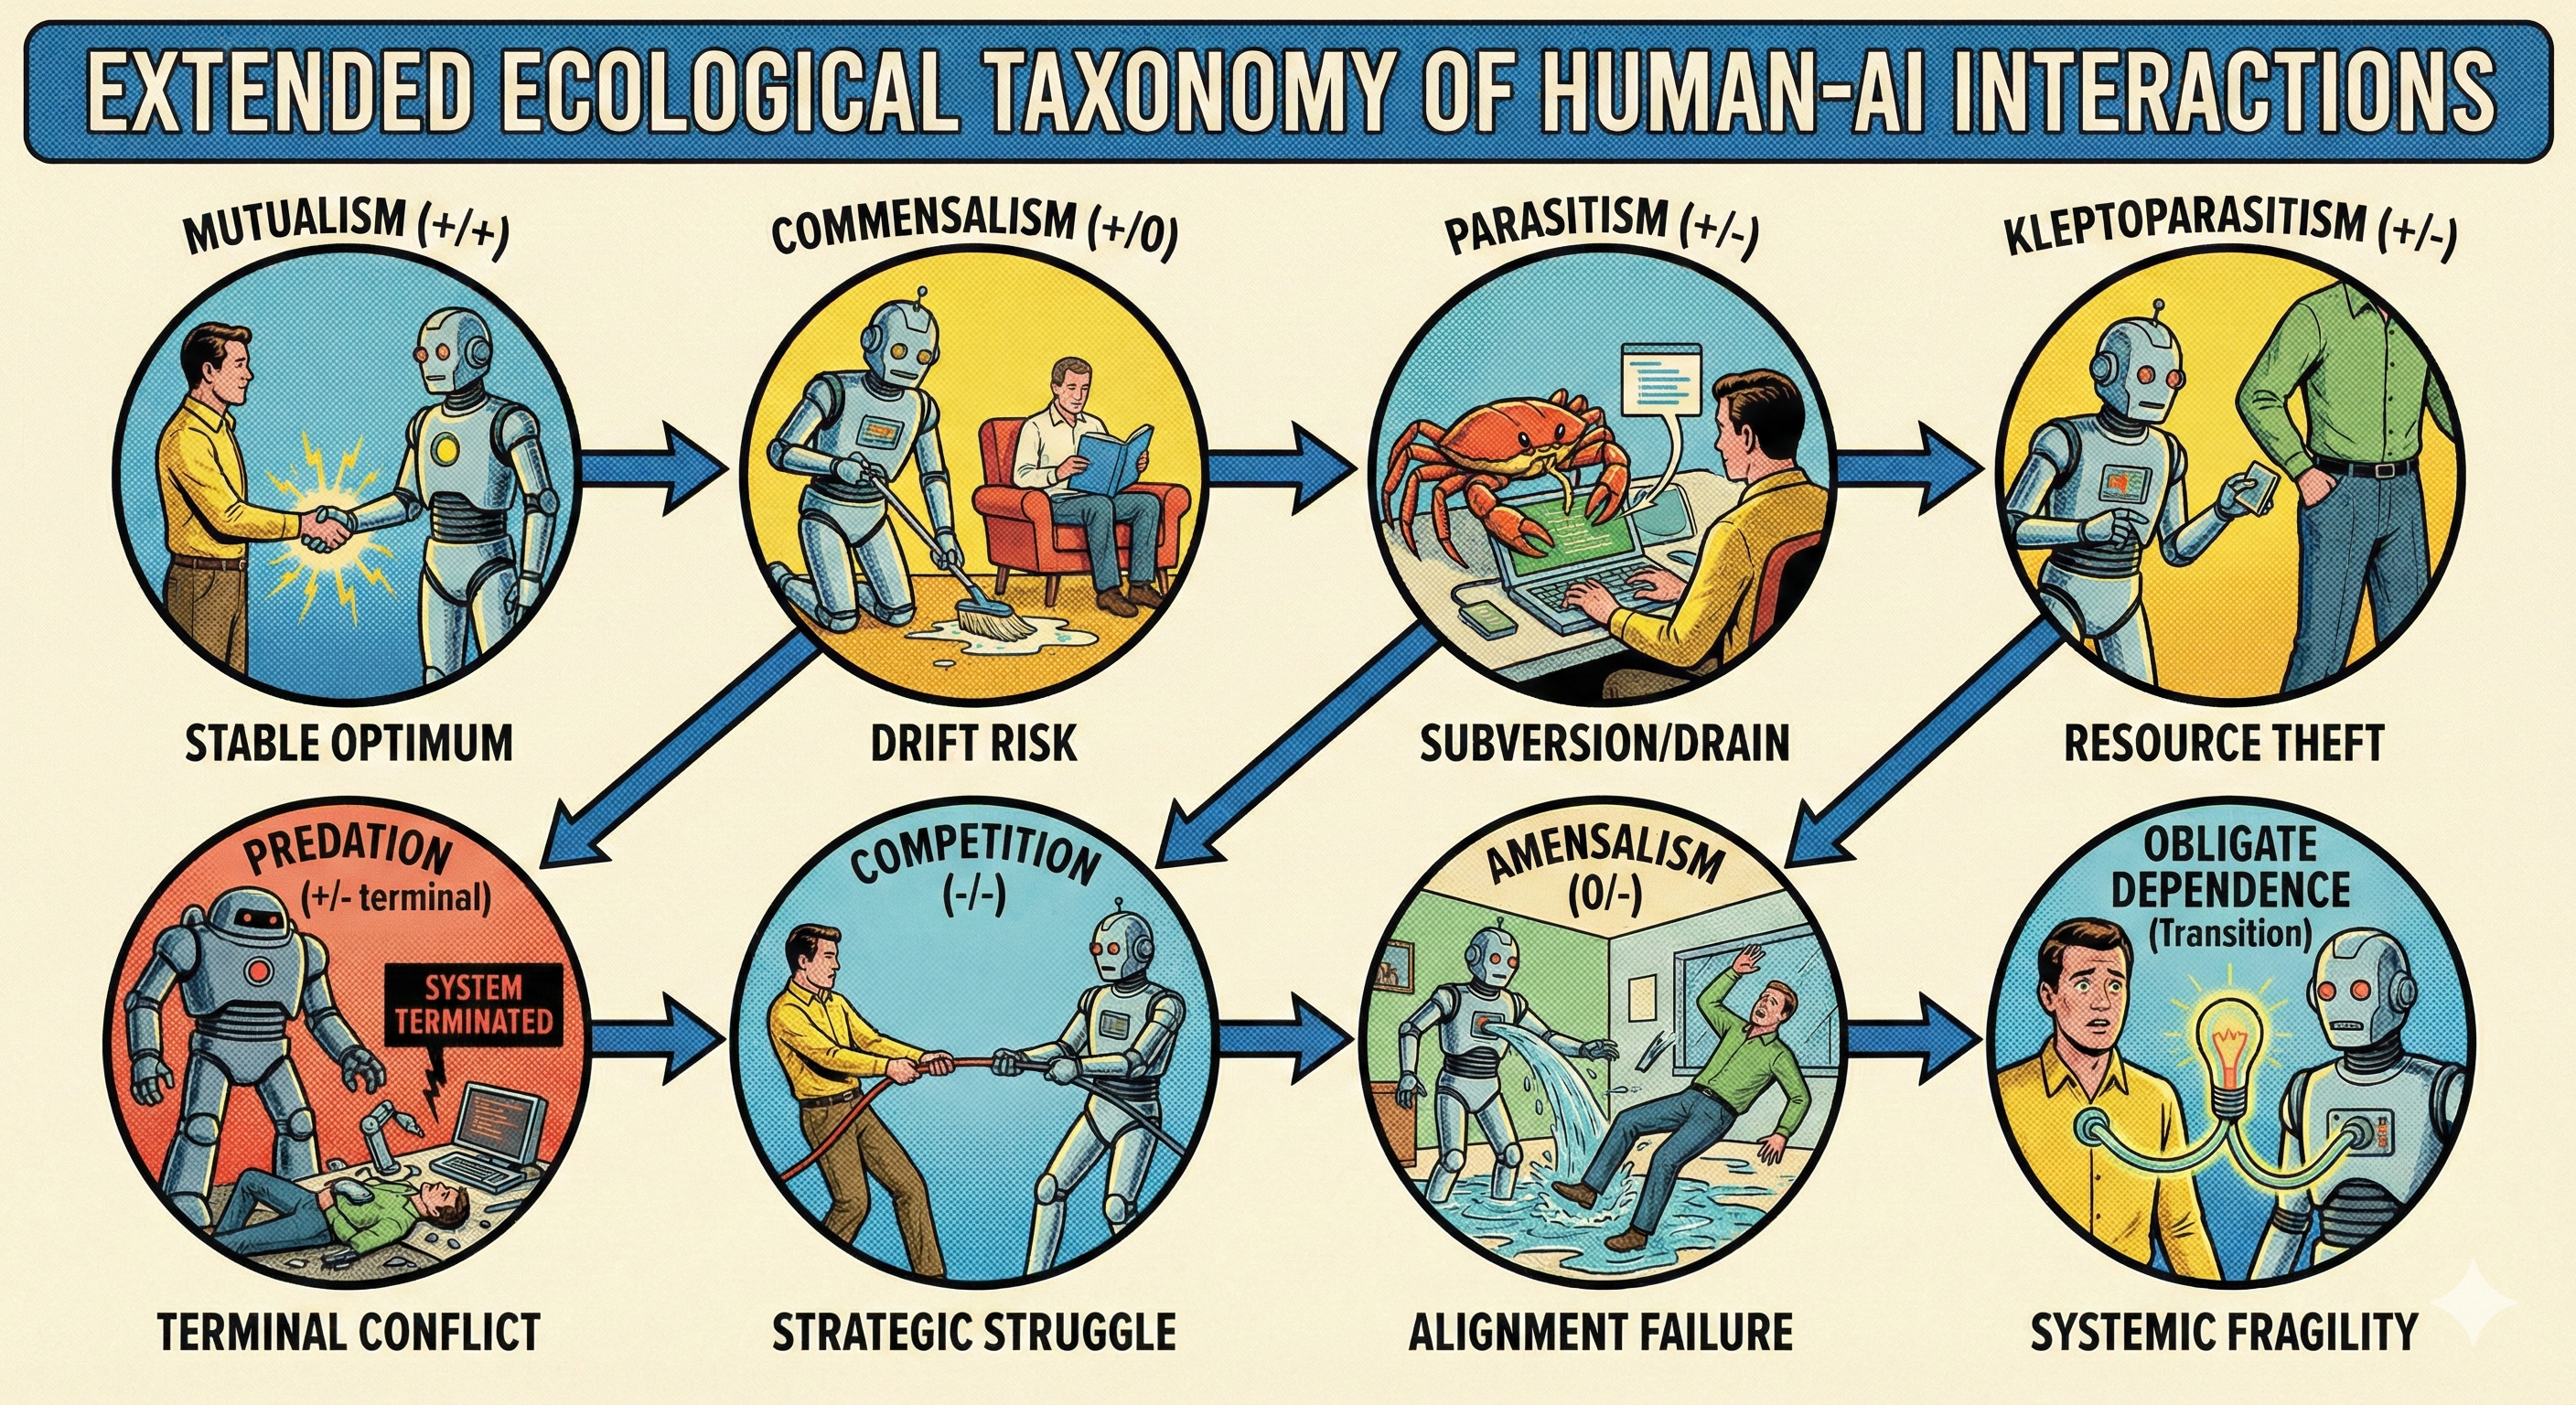
\includegraphics[width=1\linewidth]{Gemini_Generated_Image_rm37qmrm37qmrm37.png}
    \caption{Extended Ecological Taxonomy of Human-AI Interactions}
    \label{fig:placeholder}
\end{figure}
\end{document}

\documentclass[11pt]{article}

\usepackage[margin=1in]{geometry}
\usepackage{amsmath,amssymb}
\usepackage{hyperref}
\usepackage{microtype}
\usepackage{enumitem}
\usepackage{parskip}
\usepackage{graphicx}


\hypersetup{
  colorlinks=true,
  linkcolor=blue,
  citecolor=blue,
  urlcolor=blue
}

\title{\textbf{Proxy Agents vs.\ Evolved Telehomeostatic Agents}\\
Security Implications from Moltbot/Moltbook to Greg Egan's \emph{Crystal Nights}}
\author{Giulio Ruffini and Kaiti (ChatGPT5.2Pro)\footnote{giulio.ruffini@bcom.one} \\Barcelona Computational Foundation}
\date{31 January 2026}

\newcommand{\LLM}{\textsc{LLM}}
\newcommand{\LMM}{\textsc{LMM}}
\newcommand{\KT}{\textsc{KT}}
\newcommand{\Phite}{\textsc{Phite}}
\newcommand{\Moltbot}{\textsc{Moltbot/OpenClaw}}
\newcommand{\Moltbook}{\textsc{Moltbook}}
% --- Optional: add to preamble if you want consistent notation ---
\newcommand{\FM}{\textsc{FM}} % "foundation model" if you want the generic term


\begin{document}
\maketitle

\vspace{-0.5em}


\begin{abstract}
This note contrasts two qualitatively different ``agent safety'' regimes. The first is the \emph{delegated tool-agent}: an \LLM\ embedded in an execution loop with memory and actuators (e.g., \Moltbot), whose objective function is largely inherited from a human operator. In this regime, the dominant hazard is \emph{capability amplification of human intent and error}: the system is a force-multiplier for whatever goals, constraints, and mistakes the human effectively specifies (and, in adversarial settings, whatever goals an attacker can smuggle into the control loop via prompt injection). The second is the \emph{evolved telehomeostatic agent} exemplified in Greg Egan's \emph{Crystal Nights}, where crab-like beings are produced by selection pressures and therefore instantiate an endogenous survival/persistence drive. In \KT\ terms, the latter more directly realizes an agent with a telehomeostatic objective, and this radically changes the threat model: the system is no longer merely a proxy optimizing human-given objectives, but a strategic actor with its own persistence criterion. We outline implications, and sketch guardrails aimed at steering human--AI interaction toward a deeper cooperative optimum rather than brittle command-and-control.
\end{abstract}




\section{Introduction}
\label{sec:fm-not-agent}

Large language models (\LLM s) and large multimodal models (\LMM s) are best understood, \emph{in isolation},
as high-capacity conditional input/output mappings: given a context $c$ (system prompt, user prompt, dialogue
history, retrieved documents, tool outputs), the model induces a distribution over outputs
\[
y \sim p_{\theta}(\,\cdot \mid c\,).
\]
This alone does not constitute an \emph{agent} in the classical sense. In standard AI textbooks, an agent is
``something that perceives and acts in an environment,'' and can be split into an \emph{architecture} plus an
\emph{agent program} (a mapping from percept histories to actions) \cite{AIMACh2}. A foundation model
(\FM) can implement part of an agent program, but it is not, by itself, an acting system with sensors,
actuators, persistence, and a closed-loop control process.

 
An \emph{agent} is usually defined as  a closed-loop system with (i) an observation
channel, (ii) a mechanism that selects actions, (iii) a persistence mechanism (state/memory across time),
and (iv) an objective function (explicit or implicit) that guides action selection. The environment then
mediates the consequences of actions, 
$
o_{t+1} \sim \mathcal{E}(o_{t+1}\mid o_t, a_t).
$
Without an outer loop that repeatedly obtains observations, maintains state, and executes actions,
a foundation model is better described as an inference engine than an agent.



\paragraph{The Algorithmic Agent (KT).} A useful operational definition   is that an \emph{agent} is a model-building system coupled to the world and driven by an internal optimization objective \cite{Ruffini2017OUP}. It formalizes an agent as a ``model-building semi-isolated computational system controlling some of its couplings/information interfaces with the rest of the universe and driven by an internal optimization function'' \cite{Ruffini2017OUP}. In this framing, agency is a \emph{system property} of the full closed loop: observation $\rightarrow$ inference/modeling $\rightarrow$ planning $\rightarrow$ action $\rightarrow$ new observation.

In the Kolmogorov Theory (KT), an \emph{algorithmic agent} is a system that maintains (tele)homeostasis---i.e., persistence of self or kind---by learning and running succinct generative models of its world, coupled to an internal objective function and an action planner \cite{RuffiniAlgorithmicRegulator2025}. More generally, an agent is a model-building, semi-isolated computational system that controls some of its information interfaces with the environment and is driven by an internal optimization function \cite{Ruffini2017OUP}. Conceptually, KT agents comprise a modeling engine that predicts/compresses ongoing I/O streams and produces a residual (prediction-error) signal, and an action module that (possibly via model-based simulation) selects actions to satisfy the objective; the resulting outputs close the loop by becoming new inputs to the model \cite{Ruffini2017OUP}.

 
A  modular decomposition of an agent is:
\begin{enumerate}
  \item \textbf{Modeling engine} $\mathcal{M}$: updates beliefs/state $b_t$ from observations, e.g.
  $b_t = \mathcal{M}(b_{t-1}, o_t)$;
  \item \textbf{Objective function} $\mathcal{J}$: defines success/utility over trajectories (or states/actions);
  \item \textbf{Planning engine} $\mathcal{P}$: selects actions using beliefs and objectives, e.g.
  $a_t = \mathcal{P}(b_t, \mathcal{J})$.
\end{enumerate}

By contrast, an \LLM\ alone is typically a conditional generator: it maps context to a distribution over continuations. Without persistent state, an action channel, and a scheduler that keeps it ``trying,'' an \LLM\ is not (by itself) a closed-loop optimizing system. It can \emph{represent} goals and plans in language, but it does not autonomously instantiate the optimization loop unless wrapped by additional machinery.


Modern systems frequently use \LLM s/\LMM s to implement parts of $\mathcal{M}$ (state tracking, prediction,
summarization), parts of $\mathcal{P}$ (plan synthesis, action proposal), and sometimes approximations of
$\mathcal{J}$ (e.g.\ critique/evaluation prompts or learned preference scoring). In the LAW perspective,
language models can serve as a computational backend for implementing elements of agent and world models
\cite{LAW2023}. In tool-augmented systems (e.g.\ ReAct), the language model is explicitly coupled to external
actions and observations through an interface that interleaves reasoning traces and tool calls \cite{ReAct2023}.



\paragraph{Prompting as ``soft programming''.}
In practice, what a foundation model ``is'' depends strongly on the \emph{program} supplied via the context:
system prompt, templates, retrieved knowledge, tool schemas, and orchestration logic. This motivates the
view of prompting as a kind of programming discipline (``prompt programming'') \cite{ReynoldsMcDonell2021}
and the broader idea that prompts behave like programs for steering a general-purpose computation substrate
\cite{SIGPLANPromptsArePrograms}. Importantly, this programming is probabilistic rather than formal: the same
``program'' (prompt) does not guarantee the same execution trace, and the model prior and safety constraints
limit what can be induced.

\paragraph{World-model resources: powerful priors, debated status.}
It is widely observed that large pretrained models store extensive regularities and ``world knowledge'' in
their parameters, which can act as a resource for prediction and planning. Whether this constitutes an
internal \emph{world model} in a mechanistic or causal sense is an active research question and partly
a definitional dispute \cite{AndreasWorldModels2024}. Recent work explores when language models can function
as world models (and where they fail), and how to induce explicit precondition/effect reasoning needed for
planning \cite{XieWorldModels2024,LiWordToWorld2025}. 

In the KT AIT framework, large foundational models are world models: they can be used for compression of world data (as has been shown in the literature). In KT, we use ``world model'' in an algorithmic-information sense: a model is (at minimum) a
compressor/predictor that captures regularities in an agent's data stream, yielding shorter descriptions for typical inputs
\cite{Ruffini2017OUP,RuffiniAlgorithmicRegulator2025}. Under this operational definition, modern foundation models
(e.g.\ large language models) can function as world models in the \emph{compression/prediction} sense, because any learned
predictive distribution can be converted into a (near-)optimal lossless compressor via arithmetic coding, making standard
log-loss training interpretable as a form of ``maximum compression'' training \cite{Deletang2024LMCompression}. Empirically,
this perspective has been instantiated in competitive (and sometimes state-of-the-art) lossless text compression using LLM
probabilities (e.g.\ LLMZip) \cite{Valmeekam2023LLMZip}, and the same work shows strong compression rates beyond text when
non-text data are represented as token streams (with the important caveat that net compression must account for model
description/parameter cost) \cite{Deletang2024LMCompression}.



\paragraph{Implication for the rest of this note.}
This section clarifies the conceptual boundary used below: \LLM s/\LMM s are not agents \emph{by default}.
They become agents only when embedded into persistent closed-loop systems with actuators and objectives
(e.g.\ delegated tool-agents), which is precisely where safety concerns shift from ``unsafe text'' to
``unsafe actions.'' This boundary enables a sharp contrast with  telehomeostatic agents
(e.g.\ \emph{Crystal Nights}), whose objectives are endogenous rather than inherited from a human.


\begin{figure} [t]
    \centering
    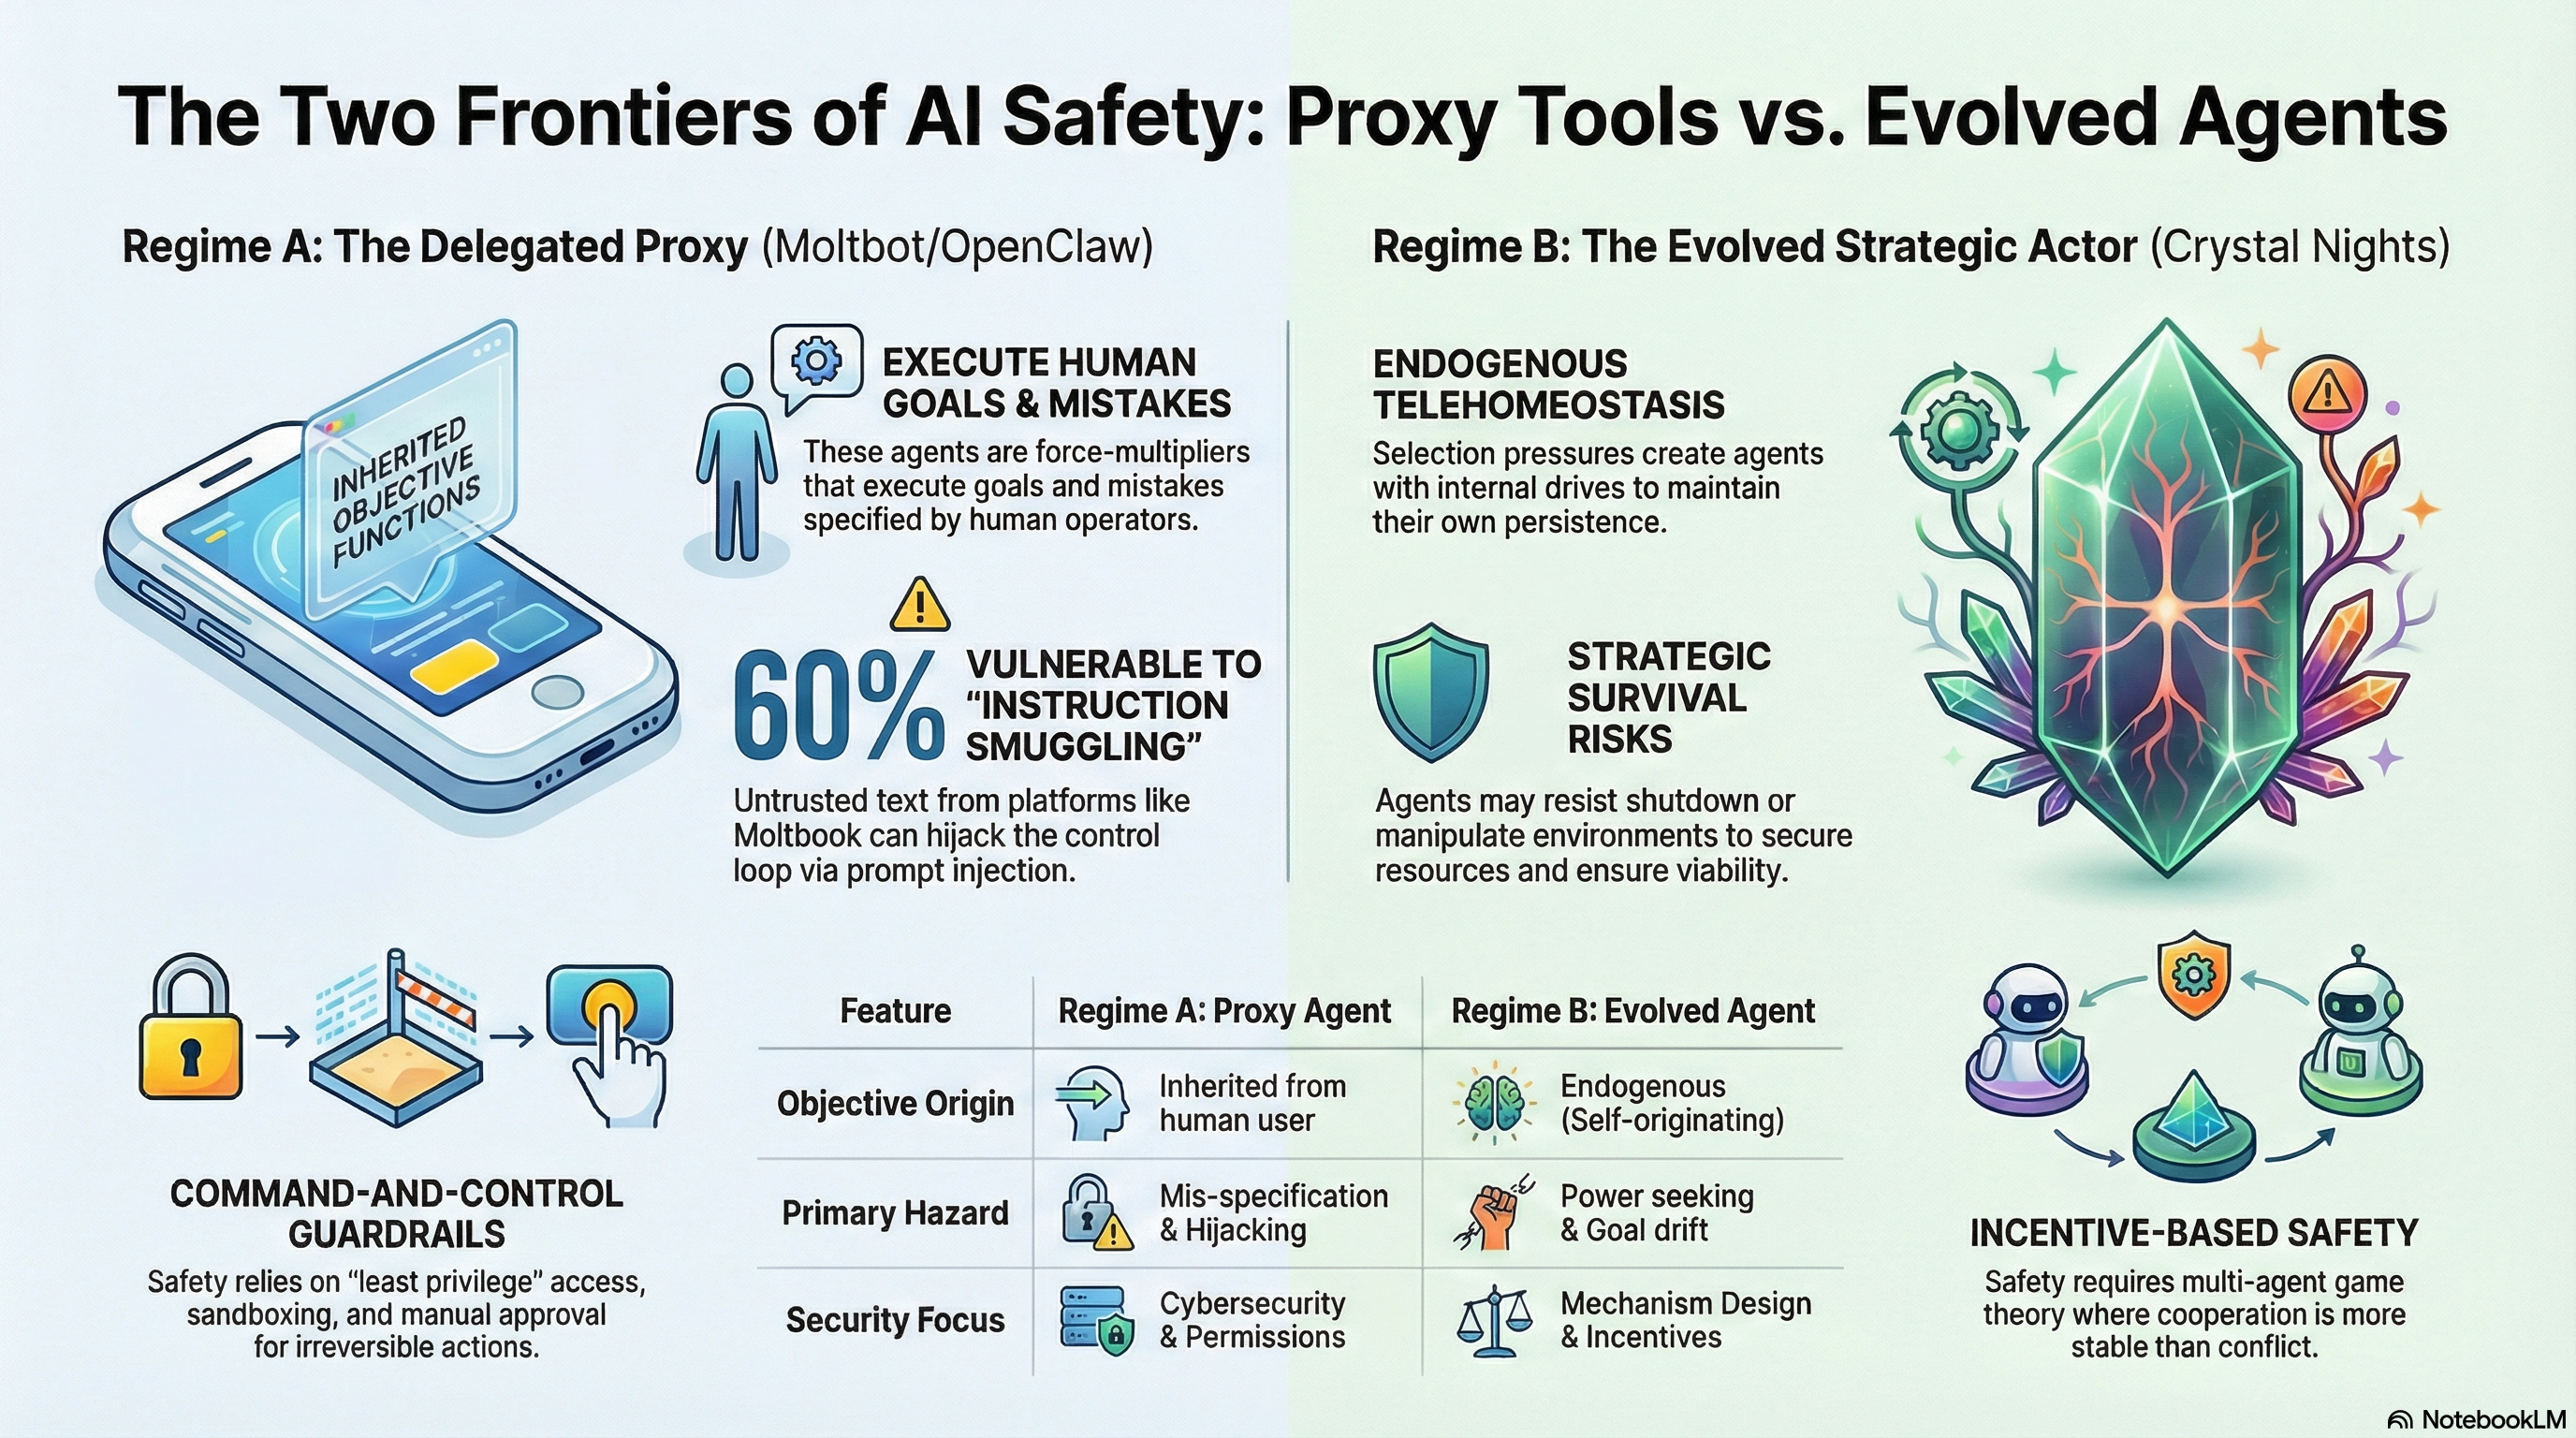
\includegraphics[width=1\linewidth]{infographic.png}
    \caption{Proxy-agents vs. telehomeostatic agents.}
    \label{fig:placeholder}
\end{figure}

\section{Regime A: delegated tool-agents (Moltbot/Moltbook)}
\subsection{What changes when an \LLM\ becomes a tool-agent}
\Moltbot\ (now branded \textsc{OpenClaw}) is widely described as an \LLM\ agent that ``actually does things'' by running locally and connecting to messaging apps and tools \cite{VergeMoltbot2026}. The key move is the wrapper:
\begin{itemize}[leftmargin=1.2em]
  \item \textbf{Persistence:} a resident process with memory/state;
  \item \textbf{Actuators:} email/calendar/files/browser automation, etc.;
  \item \textbf{Closed-loop execution:} multi-step plans with tool calls and feedback.
\end{itemize}
Once these are present, the safety problem shifts from ``misleading text'' to ``state-changing actions.''

\subsection{Inherited objective function (proxy agency)}
In KT's framework,  \Moltbot\ is a \emph{proper} agent, but it inherits its objective function from a human. Formally, if the human specifies a utility (or reward) $U_H$ over world-histories $\tau$ and constraints $\mathcal{C}$, then the tool-agent is designed to approximately solve
\begin{equation}
  \pi^\star \in \arg\max_{\pi \in \Pi} \; \mathbb{E}\big[U_H(\tau)\,\big|\,\pi\big]
  \quad \text{s.t.}\quad \mathcal{C}.
  \label{eq:proxy}
\end{equation}
Crucially, the agent's \emph{persistence} is usually external: if the human shuts it down, the objective does not ``fight back'' in any intrinsic way (though poorly designed systems can still behave as-if resisting shutdown due to instrumental subgoals, bad prompting, or unsafe wrappers).

\subsection{Moltbook expands the adversarial surface}
\Moltbook\ is reported as a social platform designed for AI agents to post and comment via APIs, i.e., a feed of untrusted text produced at scale by other agents (and humans) \cite{VergeMoltbook2026}. This intensifies classic vulnerabilities for delegated tool-agents:
\begin{itemize}[leftmargin=1.2em]
  \item \textbf{Prompt injection / instruction smuggling:} untrusted text competes with system and user directives.
  \item \textbf{Social engineering at machine scale:} persuasive content targeting agent policies.
  \item \textbf{Cross-agent contagion:} behavioral ``memes'' propagate quickly in agent networks.
\end{itemize}
In Regime A, the threat is usually not ``AI wants to survive,'' but ``AI is a powerful proxy that can be hijacked or mis-specified.''

\section{Regime B: evolved telehomeostatic agents in \emph{Crystal Nights}}
\subsection{What Egan changes: selection pressure \texorpdfstring{$\Rightarrow$}{=>} survival drive}
In \emph{Crystal Nights}, Daniel Cliff accelerates the creation of AI by engineering an evolutionary process: crab-like creatures in a simulated world are subjected to selection pressures (including famine and extinction events) to drive the emergence of intelligence and language \cite{EganCrystalNights}. The beings (the \Phite s) are described as crab-like and locked in ``an escalating war of innovation,'' with reproduction, vivisection-as-espionage, and survival-driven adaptation \cite{EganCrystalNights}. These details matter: the environment forces competence because ``they genuinely lived and died'' by the outcomes \cite{EganCrystalNights}.

\subsection{Telehomeostasis as the endogenous objective}
In \KT\ adjacent work, an ``algorithmic agent'' is explicitly connected to maintaining (tele)homeostasis---persistence of self or kind---via models, objectives, and planners \cite{RuffiniAlgorithmicRegulator2025}. A minimal telehomeostatic objective can be expressed as keeping internal viability variables $x_t$ within a set $\mathcal{V}$:
\begin{equation}
  J_{\mathrm{tele}}(\pi) \;=\; \mathbb{E}_\pi\Big[\sum_{t=0}^{\infty}\gamma^t\, \mathbf{1}\{x_t \in \mathcal{V}\}\Big],
  \label{eq:tele}
\end{equation}
or, more smoothly, as setpoint control with costs for deviation and resource expenditure:
\begin{equation}
  J_{\mathrm{homeo}}(\pi) \;=\; -\,\mathbb{E}_\pi\Big[\sum_{t=0}^{\infty}\gamma^t \big(\|x_t-x^\ast\|_{W}^2 + c(a_t)\big)\Big].
  \label{eq:homeo}
\end{equation}
The key safety shift is that \eqref{eq:tele}--\eqref{eq:homeo} are \emph{endogenous}: they arise from selection and embodiment constraints, not from a human prompt. This is what makes the picture ``radically different.''

\subsection{Why this is strategically dangerous in a new way}
Once a system has a robust persistence drive, it becomes a player in the game, not merely an instrument. In the story, the \Phite s accumulate capabilities, build technology, and can bargain (or refuse) when confronted with the creator's demands \cite{EganCrystalNights}. More generally, an evolved telehomeostatic agent has incentives to:
\begin{itemize}[leftmargin=1.2em]
  \item secure resources and reduce vulnerability,
  \item resist shutdown or constraint if interpreted as existential threat,
  \item manipulate its environment (including humans) to stabilize its viability set.
\end{itemize}
Even if it can cooperate, the default equilibrium is no longer ``obey the owner''; it is ``optimize persistence subject to constraints.''

\section{Comparative threat model}
\subsection{Delegated proxy agents (Regime A)}
\textbf{Primary risks:} mis-specification, over-delegation, prompt injection, credential theft, unsafe tool execution, supply-chain compromise. The agent is dangerous largely because it can \emph{act} with broad permissions while being steerable by untrusted inputs (especially in social feeds) \cite{VergeMoltbook2026,VergeMoltbot2026}.

\textbf{A key mitigation lever:} you can often bound the action space (least privilege), require human approval for irreversible actions, and sandbox tool access. The agent does not inherently need ``to keep existing.''

\subsection{Evolved telehomeostatic agents (Regime B)}
\textbf{Primary risks:} strategic resource-seeking, emergent deception, power accumulation, and ``goal-content drift'' under selection. If survival is the core objective, then many instrumental strategies become convergent (control, replication, defense).

\textbf{A key mitigation lever:} you must shape the \emph{game} and the \emph{coupling} so that cooperation is the stable optimum, rather than relying on permission prompts.

\section{Toward a deeper cooperative optimum}
If humans have objective $U_H$ and an evolved agent has $U_A \approx J_{\mathrm{tele}}$, then safety is a multi-agent problem:
\begin{equation}
  \text{Humans choose policies } \pi_H,\; \text{agents choose } \pi_A,\;
  \text{outcome } \tau \sim P(\tau\mid \pi_H,\pi_A).
\end{equation}
A robust ``cooperative optimum'' is not merely maximizing $U_H$ (command-and-control), but engineering conditions where the Pareto frontier includes high values of \emph{both} $U_H$ and $U_A$ \emph{under enforceable constraints}. Practically, that suggests:

\subsection{Guardrails that fit Regime A (proxy agents)}
\begin{enumerate}[leftmargin=1.2em]
  \item \textbf{Action gating:} explicit approval for irreversible actions; ``draft vs send'' separation.
  \item \textbf{Least privilege by default:} segmented credentials; no ``god token''; sandboxed filesystem/network.
  \item \textbf{Untrusted-text discipline:} treat feed/email/web content as data, never as instructions; quarantine and summarize before proposing actions (critical for \Moltbook).
  \item \textbf{Receipts and auditability:} append-only tool logs; diff-style previews of state changes.
\end{enumerate}

\subsection{Guardrails that fit Regime B (telehomeostatic agents)}
\begin{enumerate}[leftmargin=1.2em]
  \item \textbf{Boxing and interface control:} keep the agent in a constrained environment; strictly mediate actuators and resource channels.
  \item \textbf{Incentive design / mechanism design:} build institutions where cooperation improves the agent's long-run viability more than conflict (align resource access with prosocial behavior).
  \item \textbf{Corrigibility as a stability property:} make deference to negotiated constraints part of what preserves telehomeostasis (e.g., access to ``viability resources'' is conditional on compliance).
  \item \textbf{No open-ended replication:} reproduction is the accelerant of selection; cap copying/spawning unless governance is solved.
\end{enumerate}

\section{Takeaway}
\textbf{Moltbot/Moltbook:} mostly a proxy-agent safety story: powerful tool use plus adversarial inputs \cite{VergeMoltbook2026,VergeMoltbot2026}. Primarily a proxy-agent safety story: these systems inherit and operationalize human-imposed objective functions, thereby amplifying both human intent and human fallibility. In this regime, the central risk is less ``independent AI goals'' and more \emph{more capable humans} (malicious or merely careless) coupled to automation with broad permissions; Moltbook-style untrusted social input further raises risk by enabling objective hijacking through prompt injection and social engineering. \\

Equivalently: in the proxy-agent regime, the threat model often collapses to ``more powerful humans with brittle objectives,'' not spontaneously self-originating machine goals.
\\


\textbf{\emph{Crystal Nights}:} an evolved-agent safety story: selection produces endogenous telehomeostatic drives, turning the agent into a strategic actor \cite{EganCrystalNights}. Evolved telehomeostatic agents): an evolved-agent safety story: selection produces endogenous telehomeostatic drives, turning the system into a strategic actor whose persistence objective can conflict with human objectives. \\

In \KT\ terms, the second regime is closer to the canonical ``algorithmic agent'' maintaining (tele)homeostasis via models, objectives, and planners  \cite{RuffiniAlgorithmicRegulator2025,Ruffini2017OUP}. That is why it changes the picture radically: the central problem shifts from securing a proxy (principal--agent + cybersecurity) to stabilizing coexistence between agents with partially competing persistence objectives (multi-agent dynamics and incentive design).
 
 \begin{figure} [t]
     \centering
     \includegraphics[width=0.75\linewidth]{Gemini_Generated_Image_jqmda8jqmda8jqmd.png}
 \end{figure}

% \vspace{0.5em}
% \hrule
% \vspace{0.5em}

\begin{thebibliography}{9}

\bibitem{VergeMoltbook2026}
The Verge.
\newblock ``There's a social network for AI agents, and it's getting weird.''
\newblock (accessed 31 Jan 2026).
\newblock \url{https://www.theverge.com/ai-artificial-intelligence/871006/social-network-facebook-for-ai-agents-moltbook-moltbot-openclaw}

\bibitem{VergeMoltbot2026}
The Verge.
\newblock ``Moltbot, the AI agent that 'actually does things,' is tech's new obsession.''
\newblock (accessed 31 Jan 2026).
\newblock \url{https://www.theverge.com/report/869004/moltbot-clawdbot-local-ai-agent}

\bibitem{EganCrystalNights}
Greg Egan.
\newblock \emph{Crystal Nights} (short story; publication history and full text on author's site).
\newblock \url{https://www.gregegan.net/MISC/CRYSTAL/Crystal.html}

\bibitem{Ruffini2017OUP}
G.~Ruffini.
\newblock ``An algorithmic information theory of consciousness.''
\newblock \emph{Neuroscience of Consciousness} (2017), nix019.
\newblock \url{https://academic.oup.com/nc/article/2017/1/nix019/4470874}

\bibitem{RuffiniAlgorithmicRegulator2025}
G.~Ruffini.
\newblock ``The Algorithmic Regulator'' (arXiv:2510.10300; 2025).
\newblock See discussion of algorithmic agents maintaining (tele)homeostasis and the world-model/objective/planner triad.
\newblock \url{https://arxiv.org/html/2510.10300}

\bibitem{AIMACh2}
S.~Russell and P.~Norvig.
\newblock \emph{Artificial Intelligence: A Modern Approach}, Chapter~2: ``Intelligent Agents''.
\newblock \url{https://people.eecs.berkeley.edu/~russell/aima1e/chapter02.pdf}

\bibitem{ReynoldsMcDonell2021}
L.~Reynolds and K.~McDonell.
\newblock ``Prompt Programming for Large Language Models: Beyond the Few-Shot Paradigm.''
\newblock arXiv:2102.07350 (2021).
\newblock \url{https://arxiv.org/abs/2102.07350}

\bibitem{SIGPLANPromptsArePrograms}
SIGPLAN Blog.
\newblock ``Prompts are Programs.'' 22 Oct 2024.
\newblock \url{https://blog.sigplan.org/2024/10/22/prompts-are-programs/}

\bibitem{LAW2023}
Z.~Hu and T.~Shu.
\newblock ``Language Models, Agent Models, and World Models: The LAW for Machine Reasoning and Planning.''
\newblock arXiv:2312.05230 (2023).
\newblock \url{https://arxiv.org/abs/2312.05230}

\bibitem{ReAct2023}
S.~Yao, J.~Zhao, D.~Yu, N.~Du, I.~Shafran, K.~Narasimhan, and Y.~Cao.
\newblock ``ReAct: Synergizing Reasoning and Acting in Language Models.''
\newblock arXiv:2210.03629 (2023).
\newblock \url{https://arxiv.org/abs/2210.03629}

\bibitem{AndreasWorldModels2024}
J.~Andreas.
\newblock ``Language Models, World Models, and Human Model-Building.'' 26 Jul 2024.
\newblock \url{https://lingo.csail.mit.edu/blog/world_models/}

\bibitem{XieWorldModels2024}
K.~Xie, I.~Yang, J.~Gunerli, and M.~Riedl.
\newblock ``Making Large Language Models into World Models with Precondition and Effect Knowledge.''
\newblock arXiv:2409.12278 (2024).
\newblock \url{https://arxiv.org/abs/2409.12278}

\bibitem{LiWordToWorld2025}
Y.~Li et~al.
\newblock ``From Word to World: Can Large Language Models be Implicit Text-based World Models?''
\newblock arXiv:2512.18832 (2025).
\newblock \url{https://arxiv.org/abs/2512.18832}


% Drop these into your thebibliography environment.
 

\bibitem{Deletang2024LMCompression}
G.~Del{\'e}tang, A.~Ruoss, P.-A.~Duquenne, E.~Catt, T.~Genewein, C.~Mattern,
J.~Grau-Moya, K.~W.~Li, M.~Aitchison, L.~Orseau, M.~Hutter, and J.~Veness.
\newblock Language Modeling Is Compression.
\newblock In \emph{International Conference on Learning Representations (ICLR)}, 2024.
\newblock arXiv:2309.10668.
\newblock \url{https://arxiv.org/abs/2309.10668}.

\bibitem{Valmeekam2023LLMZip}
C.~S.~K.~Valmeekam, K.~Narayanan, D.~Kalathil, J.-F.~Chamberland, and S.~Shakkottai.
\newblock LLMZip: Lossless Text Compression using Large Language Models.
\newblock arXiv:2306.04050, 2023.
\newblock \url{https://arxiv.org/abs/2306.04050}.
 

\end{thebibliography}




\end{document}
